% !TEX program = xelatex
\documentclass[UTF8,fontset=fandol,a4paper,11pt]{ctexart}
\usepackage[margin=21mm,top=23mm,bottom=22mm,headheight=16pt]{geometry}
\usepackage{amsmath,amssymb,mathtools,bm}
\usepackage{tikz}
\usetikzlibrary{arrows.meta,calc,angles,quotes,patterns}
\usepackage{xcolor,booktabs,array,longtable,enumitem,fancyhdr,needspace}
\usepackage[unicode,hidelinks]{hyperref}
\definecolor{ink}{HTML}{24343C}
\definecolor{accent}{HTML}{166A70}
\definecolor{muted}{HTML}{65747A}
\definecolor{rulegray}{HTML}{D4DDE0}
\definecolor{warm}{HTML}{966037}
\color{ink}
\setlength{\parindent}{2em}
\setlength{\parskip}{4pt}
\linespread{1.12}
\AtBeginDocument{\setlength{\abovedisplayskip}{6pt plus 2pt minus 1pt}
\setlength{\belowdisplayskip}{6pt plus 2pt minus 1pt}
\setlength{\abovedisplayshortskip}{0pt plus 1pt}
\setlength{\belowdisplayshortskip}{4pt plus 1pt}}
\setlist[enumerate]{label=(\arabic*),leftmargin=2.3em,itemsep=3pt,topsep=4pt}
\setlist[itemize]{leftmargin=2em,itemsep=2pt,topsep=4pt}
\allowdisplaybreaks[1]
\setlength{\emergencystretch}{2em}
\setcounter{secnumdepth}{0}
\providecommand{\tightlist}{\setlength{\itemsep}{0pt}\setlength{\parskip}{0pt}}
\ctexset{section={format=\Large\bfseries\color{accent},beforeskip=10pt,afterskip=9pt},
subsection={format=\normalsize\bfseries\color{accent},beforeskip=10pt,afterskip=4pt},
subsubsection={format=\normalsize\bfseries,beforeskip=8pt,afterskip=3pt}}
\pagestyle{fancy}
\fancyhf{}
\fancyhead[L]{\small\color{muted}物理学难题集萃}
% 页眉仅保留书名；版本名称只在封面显示。
\fancyfoot[L]{\small\color{muted}\chapterlabel}
\fancyfoot[R]{\small\thepage}
\renewcommand{\headrulewidth}{0.4pt}
\renewcommand{\footrulewidth}{0pt}
\newcommand{\dd}{\mathop{}\!\mathrm{d}}
\newcommand{\vect}[1]{\bm{#1}}
\newcommand{\tagline}[1]{\noindent{\small\color{muted}#1}\par}
\newcommand{\result}[1]{\begin{equation*}\boxed{#1}\end{equation*}}
\newcommand{\figcaption}[1]{\par\vspace{2pt}{\small\color{muted}#1}\par}
\newcommand{\teach}[2]{\Needspace{4\baselineskip}\subsection*{讲解要点与追问}#1\par\smallskip\noindent\textbf{追问：}#2\par}
\newcommand{\workarea}{\par\vspace{7mm}\noindent{\small\color{muted}作答区}\par\vspace{4mm}
\noindent\textcolor{rulegray}{\rule{\linewidth}{0.3pt}}\par\vspace{16mm}
\noindent\textcolor{rulegray}{\rule{\linewidth}{0.3pt}}\par\vspace{16mm}
\noindent\textcolor{rulegray}{\rule{\linewidth}{0.3pt}}\par\vspace{16mm}
\noindent\textcolor{rulegray}{\rule{\linewidth}{0.3pt}}}
\tikzset{axis/.style={-{Stealth[length=2mm]},thin,color=muted},
motion/.style={-{Stealth[length=2.3mm]},thick,color=accent},
force/.style={-{Stealth[length=2.3mm]},thick,color=warm},
traj/.style={thick,color=accent},guide/.style={dashed,thin,color=muted},
object/.style={thick,color=ink},every node/.style={font=\small}}

\newcommand{\edition}{学生解答版}
\newcommand{\chapterlabel}{第一章\quad 运动学}
\hypersetup{pdftitle={第一章 运动学·学生解答版},pdfauthor={},pdfsubject={第一章第1--15题}}
\begin{document}
\pdfbookmark[0]{第一章 运动学}{cover}
\thispagestyle{empty}
\vspace*{20mm}
\noindent{\Huge\bfseries 物理学难题集萃}\par\vspace{8mm}
\noindent{\LARGE 第一章\quad 运动学}\par\vspace{10mm}
\noindent{\Large\color{accent}学生解答版}\par\vspace{8mm}
\noindent\textcolor{accent}{\rule{\linewidth}{1pt}}\par\vspace{8mm}
\noindent 第 1--15 题\par\vspace{5mm}
\noindent 完整推导、图示分析与条件讨论。\par
\vfill\clearpage
\pdfbookmark[1]{题目目录}{contents}
\section*{题目目录}
\begin{longtable}{@{}>{\color{accent}\bfseries}r p{120mm}@{}}
\toprule 题号 & 题目\\\midrule
1 & 分段运动时间比较 \\
2 & 线性阻力下的剩余路程 \\
3 & 三次阻力运动规律 \\
4 & 斜坡上的最大射程 \\
5 & 等射程抛体的飞行时间乘积 \\
6 & 水枪越墙的最小初速 \\
7 & 反弹平抛与公共越杆点 \\
8 & 导弹追踪匀速上升飞行物 \\
9 & 圆柱解线与渐开线轨迹 \\
10 & 旋转杆上小环的阿基米德螺线 \\
11 & 相对运动中的最短距离 \\
12 & 非均匀河流中的往返轨迹 \\
13 & 小船始终指向目标的河流轨迹 \\
14 & 纯滚动轮缘点速度 \\
15 & 内滚圆盘接触点加速度 \\
\bottomrule\end{longtable}


\clearpage

\pdfbookmark[2]{第 1 题 分段运动时间比较}{q1}

\section*{第 1 题\quad 分段运动时间比较}

\tagline{M-01-01}

直角三角形 $ABC$ 位于铅垂平面内，$AB$ 竖直，$BC$ 水平，$AC$ 与 $BC$ 的夹角为 $\alpha$。质点从 $A$ 点由静止出发，沿光滑约束路径在重力作用下运动到 $C$ 点。拐折不耗时，且只改变速度方向，不改变速率。
\begin{enumerate}
\item 沿 $A\to B\to C$ 的两段用时分别为 $t_1,t_2$，沿 $AC$ 用时为 $t_3$。若 $t_1+t_2=t_3$，求 $\alpha$。
\item 取上述 $\alpha$，路径限制为三角形内部及边界上的水平段与竖直段，且水平段只向右、竖直段只向下。求最短用时路径；说明如何使有限阶梯路径的用时趋近最长时间极限，并求该极限与最短用时之比。
\end{enumerate}

\begin{center}
\begin{tikzpicture}[scale=1.02]
\coordinate (A) at (0,3);\coordinate (B) at (0,0);\coordinate (C) at (4,0);
\draw[object] (A)--(B)--(C)--cycle;
\draw[motion] (0,2.6)--(0,1.2);\draw[motion] (.5,0)--(2.0,0);
\draw[motion] (.55,2.59)--(1.65,1.76);
\draw[guide] (A)--(0,2.1)--(.9,2.1)--(.9,1.4)--(1.8,1.4)--(1.8,.65)--(3.1,.65)--(3.1,0)--(C);
\draw (0,.2)--(.2,.2)--(.2,0);
\draw (3.35,0) arc[start angle=180,end angle=143.13,radius=.65];
\node at (3.1,.27) {$\alpha$};
\node[above left] at (A) {$A$};\node[below left] at (B) {$B$};\node[below right] at (C) {$C$};
\draw[force] (4.65,2.75)--(4.65,1.85) node[right] {$\vect g$};
\node[align=left,color=muted] at (6,0.9) {虚线为一条\,\\允许的阶梯路径};
\end{tikzpicture}
\figcaption{图 1.1\quad 两条比较路径与一条有限阶梯路径。示意图不按比例。}
\end{center}

\Needspace{5\baselineskip}\subsection*{解答}

设 $AC=L$，竖直高度 $h=AB=L\sin\alpha$，水平距离 $b=BC=L\cos\alpha$。解图 1.1A 中，$AB$ 是自由落体段，$BC$ 是匀速段，$AC$ 是沿光滑斜面的匀加速段。
\begin{center}\begin{minipage}{\linewidth}\centering\begin{tikzpicture}

\coordinate (A) at (0,3);\coordinate (B) at (0,0);\coordinate (C) at (4,0);
\draw[object] (A)--(B)--(C)--cycle;
\node[above left] at (A) {$A$};\node[below left] at (B) {$B$};\node[below right] at (C) {$C$};
\draw[thin,<->] (-.65,0)--(-.65,3) node[midway,left] {$L\sin\alpha$};
\draw[thin,<->] (0,-.48)--(4,-.48) node[midway,below] {$L\cos\alpha$};
\node[above right] at (2,1.5) {$L$};
\draw[motion] (0,2.6)--(0,1.55) node[midway,right] {$g$};
\draw[motion] (.55,.26)--(1.75,.26) node[midway,above] {$v_B$};
\draw[force] (2.6,1.2)--(3.55,.4875) node[midway,above right] {$g\sin\alpha$};
\draw (3.4,0) arc(180:143.13:.6);\node at (3.16,.25) {$\alpha$};
\node[align=left] at (6.2,2.2) {$AB$：自由落体\\$BC$：匀速运动\\$AC$：沿坡匀加速};

\end{tikzpicture}
\figcaption{解图 1.1A\quad 按图中的三个运动阶段分别求时间；$L=AC$。箭头分别标示加速度或速度。}
\end{minipage}\end{center}
\subsubsection*{三段时间与三角形的角度}
从静止沿 $AB$ 下落，有
\[
h=\frac12gt_1^2,\qquad
t_1=\sqrt{\frac{2L\sin\alpha}{g}},\qquad
v_B=gt_1=\sqrt{2gL\sin\alpha}.
\]
拐折只改变速度方向，所以进入 $BC$ 时速率仍为 $v_B$。水平段无沿运动方向的加速度，故
\[
t_2=\frac{b}{v_B}
=\cos\alpha\sqrt{\frac{L}{2g\sin\alpha}}.
\]
沿 $AC$ 时，重力的沿坡分量给出 $a=g\sin\alpha$，于是
\[
L=\frac12g\sin\alpha\,t_3^2,\qquad
t_3=\sqrt{\frac{2L}{g\sin\alpha}}.
\]
分别除以 $t_3$，得 $t_1/t_3=\sin\alpha$、$t_2/t_3=\cos\alpha/2$。题设因此等价于
\[
\sin\alpha+\frac12\cos\alpha=1.
\]
令 $s=\sin\alpha$，由 $0<\alpha<\pi/2$，可写 $\sqrt{1-s^2}=2(1-s)$。平方、整理得到
\[
1-s^2=4(1-2s+s^2),\qquad
(5s-3)(s-1)=0.
\]
$s=1$ 使三角形退化，舍去；$s=3/5$ 满足未平方的方程。所以
\[
\boxed{\sin\alpha=\frac35,\quad\cos\alpha=\frac45,
\quad\alpha\approx36.87^\circ}.
\]
\subsubsection*{所有竖直段的总时间相同}
第二问只允许向右的水平段和向下的竖直段。用 $z$ 表示从 $A$ 起已经下降的高度。约束力不做功，拐折不损失速率，因而任一路径上都有
\[
v(z)=\sqrt{2gz}.
\]
水平运动期间 $z$ 不变；竖直段上 $\dd t=\dd z/v(z)$。各竖直段依次覆盖 $0\leq z\leq h$，所以它们的时间相加为
\[
T_{\mathrm v}=\int_0^h\frac{\dd z}{\sqrt{2gz}}
=\sqrt{\frac{2h}{g}}=t_1.
\]
近起点的时间微元按$z^{-1/2}\dd z$变化，积分从零高度起收敛到有限时间。竖直段以哪个高度开始、分成多少段，都在同一个下降量积分中相加；路径的时间差来自水平段所在的高度。
\subsubsection*{水平段的下界与上界}
在距左边界 $x$ 的位置，三角形内部要求
\[
\frac{hx}{b}\leq z\leq h.
\]
因此每个水平微元的耗时满足
\[
\frac{\dd x}{\sqrt{2gh}}
\leq\frac{\dd x}{\sqrt{2gz}}
\leq\frac{\dd x}{\sqrt{2ghx/b}}.
\]
全部水平位移为 $b$，积分得到
\[
\frac{b}{\sqrt{2gh}}\leq T_{\mathrm h}
\leq\int_0^b\frac{\dd x}{\sqrt{2ghx/b}}
=\frac{2b}{\sqrt{2gh}}=t_1\cot\alpha.
\]
下界可达到：先沿 $AB$ 下降全部高度，再沿底边 $BC$ 走完水平距离。所以允许路径中的最短用时为
\[
T_{\min}=t_1+t_2=t_1\left(1+\frac12\cot\alpha\right)
=\frac53t_1.
\]
\begin{center}\begin{minipage}{\linewidth}\centering\begin{tikzpicture}

\draw[axis] (0,-.2)--(0,3.55) node[above] {$y$};\draw[axis] (-.2,0)--(4.7,0) node[right] {$x$};
\draw[object] (0,3)--(4,0);\node[above left] at (0,3) {$A$};\node[below left] at (0,0) {$B$};\node[below] at (4,0) {$C$};
\draw[traj] (0,3)\foreach \j in {1,...,8}{--({.5*(\j-1)},{3-.375*\j})--({.5*\j},{3-.375*\j})};
\draw[thin,<->] (1.5,1.23)--(2,1.23) node[midway,below] {$\dd x$};
\fill (1.75,1.5) circle(1.6pt);\node[above left] at (1.75,1.5) {$P$};
\draw[guide] (0,1.5)--(1.5,1.5);
\draw[thin,<->] (-.45,0)--(-.45,1.5) node[midway,left] {$y$};
\draw[thin,<->] (-1.2,1.5)--(-1.2,3) node[midway,left] {$L\sin\alpha-y$};
\draw[motion] (2.45,1.05)--(3.3,1.05) node[midway,above] {$v(y)$};
\node[align=left] at (6.6,1.5) {水平微元放得越高，\\对应速率越小，\\同样 $\dd x$ 所需时间越长。};

\end{tikzpicture}
\figcaption{解图 1.1B\quad 贴近 $AC$ 的内侧阶梯。$y$ 是距底边的高度，下降高度为 $L\sin\alpha-y$。}
\end{minipage}\end{center}
解图1.1B中的内侧阶梯用于逼近上界，水平段须尽量贴近斜边。可把总下降量分为 $N$ 份，每次先下降 $h/N$，再向右走 $b/N$；这样的阶梯始终在三角形内。其水平段总时间为
\[
T_{\mathrm h,N}=\frac{b}{\sqrt{2gh}}\,
\frac1{\sqrt N}\sum_{k=1}^N\frac1{\sqrt k}
\longrightarrow\frac{2b}{\sqrt{2gh}}.
\]
任意有限阶梯的水平段在一些非零长度的区间位于斜边下方，速率较大，用时严格小于积分给出的上确界；细分阶梯可任意逼近这一值。由 $\cot\alpha=4/3$，
\[
T_{\sup}=\frac73t_1,\qquad
\boxed{\frac{T_{\sup}}{T_{\min}}=\frac75}.
\]
这里斜边给出水平段所能接近的最高位置。每条实际路径仍由水平段和竖直段组成，所构造的是这些路径的用时极限。
\subsubsection*{图中的高度坐标与下降量}
解图1.1B使用的是离底边的高度$y$，前面使用的是累计下降量$z$，
两者满足$z=h-y$。在贴近斜边的阶梯极限上，
$x=b(1-y/h)$，故$\dd x=-(b/h)\dd y=-\cot\alpha\,\dd y$。
水平微元采用该高度处的速率$\sqrt{2g(h-y)}$；将图中的$y$换成下降量$z=h-y$后，与前面的能量关系直接衔接：
\[
T_{\mathrm h,\sup}
=-\frac{\cot\alpha}{\sqrt{2g}}
\int_h^0\frac{\dd y}{\sqrt{h-y}}
=\cot\alpha\sqrt{\frac{2h}{g}}
=\frac43t_1.
\]
从起点到终点，$y$ 由 $h$ 降至 $0$，所以 $\dd x=-\cot\alpha\,\dd y>0$。换元只改变积分的方向和微元写法，算的是同一段水平时间。

阶梯细分的收敛可由积分夹住求和来说明。对递减函数$x^{-1/2}$有
\[
2(\sqrt{N+1}-1)\leq\sum_{k=1}^Nk^{-1/2}
\leq1+2(\sqrt N-1).
\]
两边除以$\sqrt N$均趋于$2$，所以所构造阶梯的水平时间确实趋于上界。
每条有限阶梯在某些水平区间严格低于斜边，耗时严格小于上界；
这一列由水平、竖直段组成的允许路径给出用时上确界；每条有限路径的时间仍由它实际包含的运动阶段累计得到。


\Needspace{18\baselineskip}

\pdfbookmark[2]{第 2 题 线性阻力下的剩余路程}{q2}

\section*{第 2 题\quad 线性阻力下的剩余路程}

\tagline{M-01-02}

质量为 $m$ 的质点以初速度 $v_0>0$ 沿 $x$ 轴正方向运动，初始位置为 $x=0$。唯一的运动方向上的力为线性阻力 $F_x=-bv$，其中 $b>0$ 为常量。

当速度降为 $v_0/n$（$n>1$）时，求已通过路程与总路程之比。总路程指 $t\to\infty$ 时路程的极限。

\begin{center}
\begin{tikzpicture}
\draw[axis] (-.7,0)--(7.0,0) node[right] {$x$};
\fill[ink] (2.7,0) circle (2.5pt);\node[below] at (2.7,-.12) {$m$};
\draw[motion] (2.7,.4)--(4.6,.4) node[above] {$\vect v$};
\draw[force] (2.7,.4)--(1.0,.4) node[above] {$\vect F$};
\draw (0,.1)--(0,-.1);\node[below] at (0,-.1) {$O$};
\node[color=muted] at (3.4,1.25) {阻力始终与速度反向};
\end{tikzpicture}
\figcaption{图 1.2\quad 运动方向与阻力方向。}
\end{center}

\Needspace{5\baselineskip}\subsection*{解答}

取初速度方向为 $x$ 轴正向，记 $k=b/m>0$。题图 1.2 中速度向右、阻力向左，运动方程为
\[
m\dot v=-bv,\qquad\dot v=-kv,\qquad v(0)=v_0.
\]
\subsubsection*{速度与位置随时间变化}
在 $v>0$ 的运动区间内分离变量，由初始时刻积分到 $t$，
\[
\int_{v_0}^{v(t)}\frac{\dd u}{u}
=-k\int_0^t\dd s,
\qquad\ln\frac{v(t)}{v_0}=-kt.
\]
所以
\[
\boxed{v(t)=v_0e^{-kt}},\qquad
x(t)=\int_0^t v_0e^{-ks}\dd s
=\boxed{\frac{v_0}{k}(1-e^{-kt})}.
\]
速度在任意有限时刻都为正，故位移等于已通过路程。解图 1.2A 的速度曲线无限延伸，但曲线下的总面积收敛：
\begin{center}\begin{minipage}{\linewidth}\centering\begin{tikzpicture}

\draw[axis] (-.2,0)--(5,0) node[right] {$t$};\draw[axis] (0,-.15)--(0,2.65) node[above] {$v$};
\fill[accent!12] ({ln(3)},0)--plot[domain={ln(3)}:4.6,samples=70](\x,{2.2*exp(-\x)})--(4.6,0)--cycle;
\draw[traj,domain=0:4.6,samples=80] plot(\x,{2.2*exp(-\x)});
\draw[guide] ({ln(3)},0)--({ln(3)},{2.2*(1/3)})--(0,{2.2*(1/3)});
\node[left] at (0,2.2) {$v_0$};\node[left] at (0,{2.2*(1/3)}) {$v_0/n$};\node[below] at ({ln(3)},0) {$t_n$};
\node[align=left] at (6.75,1.75) {全部曲线下面积：$x_m$\\$t_n$ 后的面积：剩余路程\\$v(t)=v_0e^{-kt}$};
\draw[thin] (1.62,.25)--(3.0,1.02) node[right] {$x_m-x_n$};

\end{tikzpicture}
\figcaption{解图 1.2A\quad 速度曲线下面积等于路程；阴影部分对应速度已降至 $v_0/n$ 后的剩余路程。}
\end{minipage}\end{center}
\[
x_m=\int_0^\infty v_0e^{-kt}\dd t=\frac{v_0}{k}.
\]
$x_m$ 是无限时间下的路程极限；任意有限时刻仍有 $x<x_m,v>0$。
\subsubsection*{代入指定速度比例}
令 $v(t_n)=v_0/n$，则
\[
e^{-kt_n}=\frac1n,\qquad t_n=\frac{\ln n}{k}.
\]
此时
\[
x_n=\frac{v_0}{k}\left(1-\frac1n\right),\qquad
\boxed{\frac{x_n}{x_m}=1-\frac1n}.
\]
$n\to1^+$ 时，指定时刻趋于零，已走路程比例也趋于零；$n\to\infty$ 时，比例趋于一，所需时间却趋于无穷。
\subsubsection*{速度与位置的直接关系}
由于 $\dot v=v\,\dd v/\dd x$，运动方程还可写为
\[
v\frac{\dd v}{\dd x}=-kv.
\]
在 $v>0$ 时约去 $v$，从 $x=0,v=v_0$ 积分，得
\[
v=v_0-kx,\qquad
\boxed{\frac{v}{v_0}+\frac{x}{x_m}=1}.
\]
\begin{center}\begin{minipage}{\linewidth}\centering\begin{tikzpicture}

\draw[axis] (-.15,0)--(4.65,0) node[right] {$x$};\draw[axis] (0,-.15)--(0,2.7) node[above] {$v$};
\draw[traj] (0,2.2)--(4,0);\node[left] at (0,2.2) {$v_0$};\node[below] at (4,0) {$x_m$};
\fill ({8/3},{2.2/3}) circle(2pt);\draw[guide] ({8/3},0)--({8/3},{2.2/3})--(0,{2.2/3});
\node[below] at ({8/3},0) {$x_n$};\node[left] at (0,{2.2/3}) {$v_0/n$};
\node[align=left] at (6.7,1.65) {$\displaystyle\frac{v}{v_0}+\frac{x}{x_m}=1$\\[4pt]$x_m-x=\dfrac vk$};

\end{tikzpicture}
\figcaption{解图 1.2B\quad 消去时间后，$v$ 与 $x$ 成线性关系。由图中截距和当前点直接读出路程比例。}
\end{minipage}\end{center}
两张解图都取 $n=3$。在解图 1.2A 中，竖线经过 $kt_n=\ln3$，此处速度为 $v_0/3$。解图 1.2B 的同一时刻对应直线上的点 $(2x_m/3,v_0/3)$，距横轴截距还有 $x_m/3$。直线上任意一点的横坐标到截距的距离都是 $x_m-x=v/k$。$v$ 随时间指数衰减，随位置却线性减小；两种关系的自变量不同。
\subsubsection*{积分常数与当前状态之后的运动}
若用不定积分求位置，先得到
\[
x=-\frac{v_0}{k}e^{-kt}+C_x.
\]
将$x(0)=0$代入上式，常量项与初始指数项相抵，得到$C_x=v_0/k$。
从 $v_0$ 积到 $v$，得到 $\ln(v/v_0)$。对数的真数是速度之比，初始速度由积分下限给定。
在解图1.2A的指定时刻$t_n$之后，令$\tau=t-t_n$，
则$v(t_n+\tau)=(v_0/n)e^{-k\tau}$，因此
\[
x_m-x_n=\int_0^\infty\frac{v_0}{n}e^{-k\tau}\dd\tau
=\frac{v_0}{nk}.
\]
它恰是解图1.2B中当前点到横轴截距的水平距离。
在$t_n$之后，速度与剩余路程按同一个指数因子继续减小。每经历$\ln2/k$的时间，二者均减半；随$t\to\infty$，速度趋零，位置趋于有限的$x_m$。


\Needspace{18\baselineskip}

\pdfbookmark[2]{第 3 题 三次阻力运动规律}{q3}

\section*{第 3 题\quad 三次阻力运动规律}

\tagline{M-01-03}

质量为 $m$ 的质点以初速度 $v_0>0$ 沿 $x$ 轴正方向作直线运动，初始位置为 $x(0)=0$。唯一的运动方向上的力为 $F_x=-cv^3$，其中 $c>0$ 为常量。记 $k=c/m$。
\begin{enumerate}
\item 求速度 $v(t)$ 和位置 $x(t)$；
\item 求速度随位置的变化规律 $v(x)$；
\item 判断总路程是否有限，并说明理由。
\end{enumerate}

\begin{center}
\begin{tikzpicture}
\draw[axis] (-.4,0)--(7.0,0) node[right] {$x$};
\fill[ink] (3,0) circle (2.5pt);\node[below] at (3,-.12) {$m$};
\draw[motion] (3,.4)--(4.6,.4) node[above] {$\vect v$};
\draw[force] (3,.4)--(1.3,.4) node[above] {$F_x=-cv^3$};
\node[color=muted] at (3.4,1.35) {规定 $x(0)=0,\quad v(0)=v_0$};
\draw (0,.1)--(0,-.1);\node[below] at (0,-.1) {$O$};
\end{tikzpicture}
\figcaption{图 1.3\quad 初始速度沿正方向，三次阻力沿负方向。}
\end{center}

\Needspace{5\baselineskip}\subsection*{解答}

记 $k=c/m$。初速度为正，阻力与运动方向相反，故
\[
\dot v=-kv^3,\qquad v(0)=v_0>0,\qquad x(0)=0.
\]
\subsubsection*{分离变量求速度}
质点以 $v_0>0$ 出发。在速度保持为正的区间分离变量：
\[
\int_{v_0}^{v(t)}u^{-3}\dd u=-k\int_0^t\dd s,
\qquad -\frac1{2v^2}+\frac1{2v_0^2}=-kt.
\]
因此
\[
\frac1{v^2}=\frac1{v_0^2}+2kt,
\qquad\boxed{v(t)=\frac{v_0}{\sqrt{1+2kv_0^2t}}}.
\]
初速度沿正方向，故取正根。任意有限时刻都有$v(t)>0$，质点一直向右，$x(t)$也是从出发起走过的路程。
\subsubsection*{积分求位置}
由 $\dot x=v(t)$，
\[
x(t)=\int_0^t\frac{v_0\dd s}{\sqrt{1+2kv_0^2s}}.
\]
令 $u=1+2kv_0^2s$，则 $\dd u=2kv_0^2\dd s$，上下限为 $1$ 与 $1+2kv_0^2t$。于是
\[
x(t)=\frac1{2kv_0}\int_1^{1+2kv_0^2t}u^{-1/2}\dd u
=\boxed{\frac{\sqrt{1+2kv_0^2t}-1}{kv_0}}.
\]
\begin{center}\begin{minipage}{\linewidth}\centering\begin{tikzpicture}

\begin{scope}
\draw[axis] (-.1,0)--(4.6,0) node[right] {$q$};\draw[axis] (0,-.1)--(0,2.6) node[above] {$v/v_0$};
\draw[traj,domain=0:4.2,samples=80] plot(\x,{2.1/sqrt(1+2*\x)});\node[left] at (0,2.1) {$1$};
\node[below] at (2,-.55) {$q=kv_0^2t$};\node at (2.5,2.25) {速率趋于零};
\end{scope}
\begin{scope}[xshift=6.7cm]
\draw[axis] (-.1,0)--(4.6,0) node[right] {$q$};\draw[axis] (0,-.1)--(0,2.6) node[above] {$kv_0x$};
\draw[traj,domain=0:4.2,samples=80] plot(\x,{sqrt(1+2*\x)-1});
\node[below] at (2,-.55) {$q=kv_0^2t$};\node at (2.2,2.65) {位移仍不断增加};
\end{scope}

\end{tikzpicture}
\figcaption{解图 1.3A\quad 两图使用同一无量纲时间 $q$。左图尾部衰减很慢，右图没有有限位移上界。}
\end{minipage}\end{center}
解图 1.3A 左图的纵坐标是$v/v_0$，右图是$kv_0x$。由于$\dd(kv_0x)/\dd q=v/v_0$，左图从0到$q$的面积就是右图在$q$处的纵坐标。右图的斜率随左图的速率减小，位置仍持续增长。
\subsubsection*{速度随位置的关系}
由位置式先得 $\sqrt{1+2kv_0^2t}=1+kv_0x$，再代入速度式，得到
\[
\boxed{v(x)=\frac{v_0}{1+kv_0x}},\qquad x\geq0.
\]
也可直接换自变量：
\[
v\frac{\dd v}{\dd x}=-kv^3
\quad\Longrightarrow\quad
\int_{v_0}^{v}\frac{\dd u}{u^2}=-k\int_0^x\dd\xi.
\]
积分后 $-1/v+1/v_0=-kx$，仍得到同一结果。约去 $v$ 的步骤只在正速度区间内使用。
\subsubsection*{初始条件、量纲和长期路程}
将 $t=0$ 代入，确有 $v=v_0,x=0$。$[k]=\mathrm{s/m^2}$，故 $kv_0^2t$、$kv_0x$ 均无量纲，而 $1/(kv_0)$ 是长度。弱阻力展开为
\[
v(t)=v_0-kv_0^3t+O(k^2),\qquad
x(t)=v_0t-\frac12kv_0^3t^2+O(k^2).
\]
这与初始加速度 $-kv_0^3$ 一致。在大时间下，
\[
v(t)\sim\frac1{\sqrt{2kt}},\qquad
x(t)\sim\sqrt{\frac{2t}{k}}\longrightarrow\infty.
\]
总路程无界。解图 1.3A 左图的尾部随$t^{-1/2}$衰减，面积随$\sqrt t$增长。右图逐渐变缓的曲线正是这段面积累积后的结果。

\Needspace{18\baselineskip}

\pdfbookmark[2]{第 4 题 斜坡上的最大射程}{q4}

\section*{第 4 题\quad 斜坡上的最大射程}

\tagline{M-01-04}

一门大炮位于倾角为 $\theta$ 的笔直山坡上，其中 $0\leq\theta<\pi/2$。炮弹在沿山坡上升方向的铅垂截面内发射，初速为 $v_0$，炮口方向相对山坡的仰角为 $\alpha$，且 $0<\alpha<\pi/2-\theta$。忽略空气阻力。
\begin{enumerate}
\item 取炮口为原点，水平向右为 $x$ 轴、竖直向上为 $y$ 轴，求落点坐标及沿坡射程 $R$；
\item 求使 $R$ 最大的仰角 $\alpha$ 及最大射程。
\end{enumerate}

\begin{center}
\begin{tikzpicture}[scale=1.08]
\draw[axis] (-.4,0)--(6.2,0) node[right] {$x$};\draw[axis] (0,-.3)--(0,3.4) node[above] {$y$};
\draw[object] (0,0)--(5.8,1.74) node[right] {山坡};
\draw[traj,domain=0:4.5,samples=70] plot (\x,{(10/7)*\x-((10/7)-.3)*\x*\x/4.5});
\draw[motion] (0,0)--(.98,1.4) node[above] {$\vect v_0$};
\draw[thin] (1.1,0) arc (0:16.699:1.1);\node at (1.37,.17) {$\theta$};
\draw[thin] (.7663,.2299) arc (16.699:55.008:.8);\node at (1.02,.76) {$\alpha$};
\fill (4.5,1.35) circle (1.8pt);\node[above right] at (4.5,1.35) {$P$};
\draw[guide] (4.5,1.35)--(4.5,0);\node[below] at (4.5,0) {$x_f$};\node[below left] at (0,0) {$O$};
\draw[thin,<->] (.2,-.35)--(4.7,1.0) node[midway,below,sloped] {$R$};
\end{tikzpicture}
\figcaption{图 1.4\quad $\alpha$ 从坡面量起，水平发射角为 $\theta+\alpha$。}
\end{center}

\Needspace{5\baselineskip}\subsection*{解答}

炮口方向与水平线的夹角为 $\beta=\theta+\alpha$。解图 1.4A 中，$\theta$ 是坡角，$\alpha$ 从山坡向上量起。题设角度区间保证 $\cos\beta>0$，飞行中$x$随$t$增大，落点在炮口右侧。解图1.4A中的$P$是炮弹再次到达坡线的位置。
\begin{center}\begin{minipage}{\linewidth}\centering\begin{tikzpicture}

\draw[axis] (-.25,0)--(5.4,0) node[right] {$x$};\draw[axis] (0,-.3)--(0,3.35) node[above] {$y$};
\draw[object] (0,0)--(5.3,1.59) node[right] {坡面};
\draw[traj,domain=0:4.5,samples=70] plot(\x,{(10/7)*\x-((10/7)-.3)*\x^2/4.5});
\fill (4.5,1.35) circle(1.8pt) node[below right] {$P$};
\draw[guide] (4.5,1.35)--(4.5,0) node[below] {$x_f$};
\draw[motion] (0,0)--(1.4,2.0) node[above] {$v_0$};
\draw[motion] (0,0)--(1.4,0) node[midway,below] {$v_0\cos\beta$};
\draw[motion] (0,0)--(0,2) node[midway,left] {$v_0\sin\beta$};
\draw[guide] (0,2)--(1.4,2)--(1.4,0);
\draw (.6,0) arc(0:55:.6);\node at (.88,.5) {$\beta$};
\draw (1.6,0) arc(0:16.699:1.6);\node at (1.8,.25) {$\theta$};
\node[align=left,anchor=west] at (3.25,2.88) {$\beta=\theta+\alpha$\\$P$处$y_f=x_f\tan\theta$};

\end{tikzpicture}
\figcaption{解图 1.4A\quad 先把坡面仰角转换为水平发射角，再按水平、竖直方向分解初速度。}
\end{minipage}\end{center}
\subsubsection*{轨迹与落点相交条件}
在水平、竖直坐标中，
\[
x=v_0\cos\beta\,t,\qquad
y=v_0\sin\beta\,t-\frac12gt^2.
\]
山坡为 $y=x\tan\theta$。代入并整理，
\[
t\left[v_0(\sin\beta-\cos\beta\tan\theta)-\frac12gt\right]=0.
\]
$t=0$ 是发射时刻，落点取正根。由
\[
\sin\beta-\cos\beta\tan\theta
=\frac{\sin(\beta-\theta)}{\cos\theta}
=\frac{\sin\alpha}{\cos\theta},
\]
得到飞行时间
\[
t_f=\frac{2v_0\sin\alpha}{g\cos\theta}.
\]
所以落点坐标和沿坡射程为
\[
\boxed{x_f=\frac{2v_0^2\cos(\theta+\alpha)\sin\alpha}{g\cos\theta},
\quad y_f=x_f\tan\theta},
\]
\[
\boxed{R=\frac{x_f}{\cos\theta}
=\frac{2v_0^2\cos(\theta+\alpha)\sin\alpha}{g\cos^2\theta}}.
\]
同一结果也可由轨迹方程与坡线求第二交点得到：
\[
y=x\tan\beta-\frac{gx^2}{2v_0^2\cos^2\beta},\qquad
x_f=\frac{2v_0^2\cos^2\beta}{g}(\tan\beta-\tan\theta).
\]
这里舍去的是炮口交点 $x=0$。
\subsubsection*{用沿坡与法向坐标求飞行时间}
解图 1.4B 中取 $s$ 沿坡向上、$n$ 垂直坡向外。重力的两个分量给出
\begin{center}\begin{minipage}{\linewidth}\centering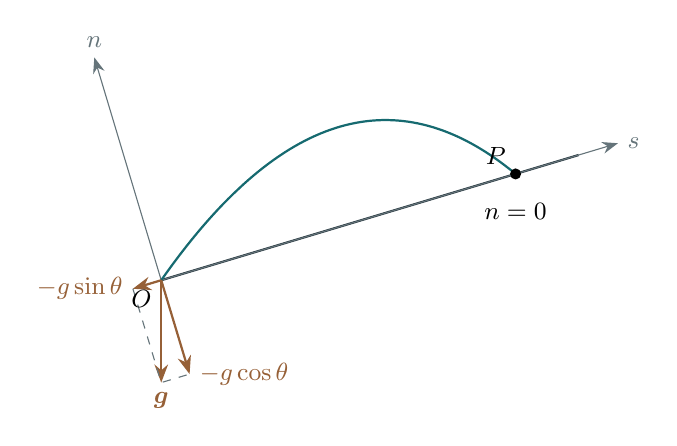
\begin{tikzpicture}

\draw[object] (0,0)--(5.3,1.59);
\draw[axis] (-.3,-.09)--(5.8,1.74) node[right] {$s$};
\draw[axis] (.09,-.3)--(-.85,2.83) node[above] {$n$};
\draw[traj,domain=0:4.5,samples=70] plot(\x,{(10/7)*\x-((10/7)-.3)*\x^2/4.5});
\fill (4.5,1.35) circle(2pt);\node[above left] at (4.5,1.35) {$P$};\node[below] at (4.5,1.10) {$n=0$};
\draw[force] (0,0)--(0,-1.3) node[below] {$\vect g$};
\draw[force] (0,0)--(-.36,-.108) node[left] {$-g\sin\theta$};
\draw[force] (0,0)--(.36,-1.192) node[right] {$-g\cos\theta$};
\draw[guide] (-.36,-.108)--(0,-1.3)--(.36,-1.192);
\node[below left] at (0,0) {$O$};

\end{tikzpicture}
\figcaption{解图 1.4B\quad 沿坡与垂直坡面建立坐标，飞行终点的条件变为 $n=0$。}
\end{minipage}\end{center}
\[
s=v_0\cos\alpha\,t-\frac12g\sin\theta\,t^2,
\qquad n=v_0\sin\alpha\,t-\frac12g\cos\theta\,t^2.
\]
由第二次 $n=0$ 得到同一 $t_f$；将它代入 $s$，展开后为
\[
R=\frac{2v_0^2\sin\alpha}{g\cos^2\theta}
(\cos\alpha\cos\theta-\sin\alpha\sin\theta),
\]
即上面的射程式。
\subsubsection*{求最优角}
用积化和差公式，
\[
2\sin\alpha\cos(\theta+\alpha)
=\sin(\theta+2\alpha)-\sin\theta.
\]
因而
\[
R(\alpha)=\frac{v_0^2}{g\cos^2\theta}
[\sin(\theta+2\alpha)-\sin\theta].
\]
在题设区间内，$\theta+2\alpha$ 可取 $\pi/2$；正弦的最大值为一，故
\[
\boxed{\alpha_*=\frac\pi4-\frac\theta2},\qquad
\boxed{R_{\max}=\frac{v_0^2(1-\sin\theta)}{g\cos^2\theta}
=\frac{v_0^2}{g(1+\sin\theta)}}.
\]
水平仰角则为 $\beta_* =\pi/4+\theta/2$。$\theta=0$ 时恢复水平地面的 $45^\circ$ 与 $v_0^2/g$；$\theta\to\pi/2^-$ 时沿坡最大射程趋于 $v_0^2/(2g)$，水平射程趋于零。
\subsubsection*{对落点横坐标求导的另一方法}
固定坡角时，解图1.4A中的$x_f$与沿坡射程$R$只相差正因子$\cos\theta$，
所以两者在同一发射角处取最大值。将第二交点写为
\[
x_f=\frac{v_0^2}{g}
\left[\sin2\beta-2\tan\theta\cos^2\beta\right],
\qquad \beta=\theta+\alpha,
\]
对$\alpha$求导时$\dd\beta/\dd\alpha=1$，从而
\[
\frac{\dd x_f}{\dd\alpha}
=\frac{2v_0^2}{g}
[\cos2\beta+\tan\theta\sin2\beta]
=\frac{2v_0^2}{g\cos\theta}\cos(2\beta-\theta).
\]
允许区间内的零点为$2\beta-\theta=\pi/2$，即
$\alpha=\pi/4-\theta/2$；从小仰角逐渐抬高炮口时，$x_f$先增加，越过这个角度后减小。
当$\alpha$趋近区间两端时，第二交点都回到炮口，射程趋于零，
这个内部驻点给出最大射程。求导还能说明从小仰角继续抬高时，落点怎样先远离炮口再返回。


\Needspace{18\baselineskip}

\pdfbookmark[2]{第 5 题 等射程抛体的飞行时间乘积}{q5}

\section*{第 5 题\quad 等射程抛体的飞行时间乘积}

\tagline{M-01-05}

两质点从同一水平地面上的同一点，以相同速率 $v_0$、不同仰角 $\alpha_1$ 和 $\alpha_2$ 抛出，且 $0<\alpha_1,\alpha_2<\pi/2$。两质点均落回该水平地面，空气阻力忽略。

若两次抛射的射程同为 $R$，证明两次飞行时间满足
\[
T_1T_2=\frac{2R}{g}.
\]

\begin{center}
\begin{tikzpicture}[x=1cm,y=1cm]
\draw[axis] (-.35,0)--(6.5,0) node[right] {$x$};\draw[axis] (0,-.2)--(0,3.5) node[above] {$y$};
\draw[traj,domain=0:6,samples=70] plot (\x,{1.73205*\x*(1-\x/6)});
\draw[traj,dashed,domain=0:6,samples=70] plot (\x,{.57735*\x*(1-\x/6)});
\draw[motion] (0,0)--(.6,1.039);\draw[motion] (0,0)--(1.039,.6);
\draw (.7,0) arc(0:30:.7);\node at (1,.22) {$\alpha_1$};
\draw (1.0,0) arc(0:60:1);\node at (1.05,1.05) {$\alpha_2$};
\node[color=accent] at (4.2,2.7) {高轨迹};\node[color=accent] at (4.5,.95) {低轨迹};
\fill (6,0) circle (1.8pt);\node[below] at (6,-.05) {$R$};\node[below left] at (0,0) {$O$};
\end{tikzpicture}
\figcaption{图 1.5\quad 同初速、同射程的两条不同轨迹。}
\end{center}

\Needspace{5\baselineskip}\subsection*{解答}

题图 1.5 的两条轨迹从同一点出发并落到同一水平地面。低角度轨迹的水平速度较大，高角度轨迹的竖直初速度较大；先由落地条件分别求时间和射程。
\subsubsection*{单次抛射的时间与射程}
对仰角为 $\alpha$ 的一次运动，
\[
x=v_0\cos\alpha\,t,\qquad
y=v_0\sin\alpha\,t-\frac12gt^2.
\]
落回地面时 $y=0$。舍去发射根 $t=0$ 后，
\[
T=\frac{2v_0\sin\alpha}{g},\qquad
R=v_0\cos\alpha\,T=\frac{v_0^2}{g}\sin2\alpha.
\]
\subsubsection*{等射程的两角互余}
初速相同、射程相同，故 $\sin2\alpha_1=\sin2\alpha_2$。将差化为乘积，
\[
2\cos(\alpha_1+\alpha_2)\sin(\alpha_1-\alpha_2)=0.
\]
两角均在 $(0,\pi/2)$ 且不同，所以 $\sin(\alpha_1-\alpha_2)\ne0$，只能有
\[
\boxed{\alpha_1+\alpha_2=\frac\pi2}.
\]
\begin{center}\begin{minipage}{\linewidth}\centering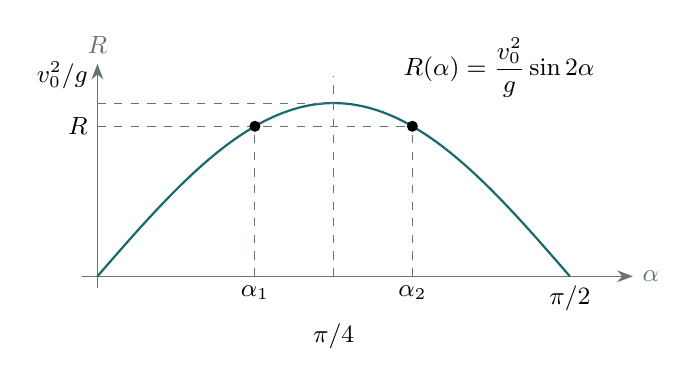
\begin{tikzpicture}

\draw[axis] (-.2,0)--(6.8,0) node[right] {$\alpha$};\draw[axis] (0,-.15)--(0,2.7) node[above] {$R$};
\draw[traj,domain=0:6,samples=90] plot(\x,{2.2*sin(30*\x)});
\draw[guide] (0,{2.2*sin(60)})--(4,{2.2*sin(60)});\node[left] at (0,{2.2*sin(60)}) {$R$};
\draw[guide] (0,2.2)--(3,2.2);\node[above left,yshift=1.5pt] at (0,2.2) {$v_0^2/g$};
\draw[guide] (2,0)--(2,{2.2*sin(60)});\draw[guide] (4,0)--(4,{2.2*sin(60)});
\fill (2,{2.2*sin(60)}) circle(2pt);\fill (4,{2.2*sin(60)}) circle(2pt);
\node[below] at (2,0) {$\alpha_1$};\node[below] at (4,0) {$\alpha_2$};\node[below] at (6,0) {$\pi/2$};
\draw[guide] (3,0)--(3,2.55);\node[below] at (3,-.48) {$\pi/4$};
\node at (5.1,2.65) {$R(\alpha)=\dfrac{v_0^2}{g}\sin2\alpha$};

\end{tikzpicture}
\figcaption{解图 1.5A\quad 射程曲线关于 $\alpha=\pi/4$ 对称；同一射程的两个不同仰角互余。}
\end{minipage}\end{center}
解图 1.5A 中，两条竖虚线从同一射程水平线落到横轴，读得一低一高的两个角。它们到 $45^\circ$ 的距离相同。射程升至 $v_0^2/g$ 时，两交点合为顶点，对应唯一的 $45^\circ$ 发射角。
\subsubsection*{求飞行时间乘积}
分别写出两次飞行时间并相乘，
\[
T_1T_2=\frac{4v_0^2}{g^2}\sin\alpha_1\sin\alpha_2
=\frac{4v_0^2}{g^2}\sin\alpha_1\cos\alpha_1
=\frac{2v_0^2}{g^2}\sin2\alpha_1.
\]
由 $R=v_0^2\sin2\alpha_1/g$，得到
\[
\boxed{T_1T_2=\frac{2R}{g}}.
\]
从时间式看，低角度的竖直初速度较小，所以先回到地面。两次飞行时间的乘积由共同射程确定。$R/g$ 的量纲是时间平方。等高落地使两次时间都等于各自竖直初速度的 $2/g$ 倍，互余角又让这两个竖直分量恰好等于一次发射里的水平、竖直分量。
\subsubsection*{共同对称轴与两个顶点的高度}
消去时间并使用落点 $x=R,y=0$，任一轨迹可改写为
\[
y=x\tan\alpha\left(1-\frac{x}{R}\right).
\]
最高点都在 $x=R/2$，高度为 $H_i=R\tan\alpha_i/4$。因为两角互余，$\tan\alpha_1\tan\alpha_2=1$，所以
\[
H_1H_2=\frac{R^2}{16}.
\]
题图 1.5 中，两个最高点沿 $x=R/2$ 竖直对齐。每个质点从最高点以零竖直速度下落，经过 $T_i/2$ 到达地面，因此 $H_i=gT_i^2/8$。这给出 $T_1T_2=(8/g)\sqrt{H_1H_2}=2R/g$。读出两顶点的高度，还可用 $T_2/T_1=\sqrt{H_2/H_1}$ 比较飞行时间。

\Needspace{18\baselineskip}

\pdfbookmark[2]{第 6 题 水枪越墙的最小初速}{q6}

\section*{第 6 题\quad 水枪越墙的最小初速}

\tagline{M-01-06}

地面上的水枪枪口视为质点，与竖直墙的水平距离为 $d=3.0\,\mathrm m$，墙高为 $h=4.0\,\mathrm m$。水流以速率 $v_0$、仰角 $\alpha$ 喷出，忽略空气阻力和水流宽度，取 $g=10\,\mathrm{m/s^2}$。

求使水流恰好通过墙顶的最小初速及相应仰角。

\begin{center}
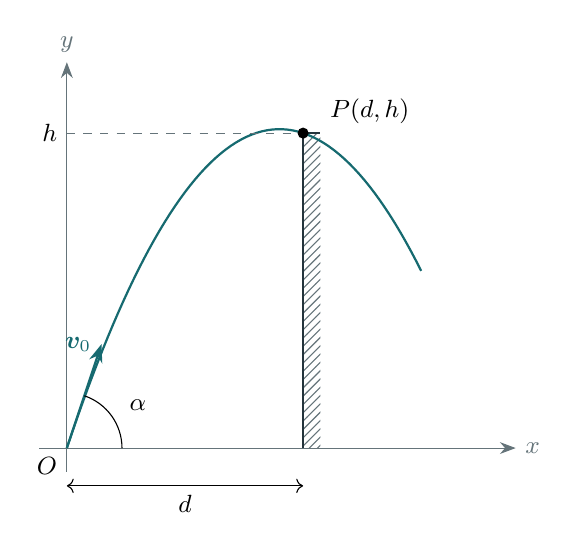
\begin{tikzpicture}[scale=1.0]
\draw[axis] (-.35,0)--(5.7,0) node[right] {$x$};\draw[axis] (0,-.3)--(0,4.9) node[above] {$y$};
\fill[pattern=north east lines,pattern color=muted] (3,0) rectangle (3.22,4);
\draw[object] (3,0)--(3,4)--(3.22,4);
\draw[traj,domain=0:4.5,samples=70] plot(\x,{3*\x-5*\x*\x/9});
\draw[motion] (0,0)--(.44,1.32) node[left] {$\vect v_0$};
\draw (.7,0) arc(0:71.565:.7);\node at (.9,.55) {$\alpha$};
\draw[guide] (0,4)--(3,4);\node[left] at (0,4) {$h$};
\draw[thin,<->] (0,-.48)--(3,-.48) node[midway,below] {$d$};
\fill (3,4) circle (2pt);\node[above right] at (3.22,4) {$P(d,h)$};\node[below left] at (0,0) {$O$};
\end{tikzpicture}
\figcaption{图 1.6\quad 枪口、墙顶与一条通过墙顶的轨迹。}
\end{center}

\Needspace{5\baselineskip}\subsection*{解答}

以枪口为原点，水平向墙为 $x$ 正向，竖直向上为 $y$ 正向。墙顶坐标为 $(d,h)$，解图 1.6A 中从枪口指向墙顶的直线与水平夹角记为 $\theta$，故 $\tan\theta=h/d$。
\begin{center}\begin{minipage}{\linewidth}\centering\begin{tikzpicture}

\draw[axis] (-.2,0)--(4.1,0) node[right] {$x$};\draw[axis] (0,-.2)--(0,4.6) node[above] {$y$};
\draw[object] (3,0)--(3,4);\fill (3,4) circle(2pt);\node[above right] at (3,4) {$P(d,h)$};
\draw[guide] (0,0)--(3,4) node[midway,above left,sloped] {$\sqrt{d^2+h^2}$};
\draw[motion] (0,0)--(.65,1.95) node[left] {$v_0$};
\draw (.68,0) arc(0:71.565:.68);\node at (.88,.7) {$\alpha$};
\draw (1.35,0) arc(0:53.13:1.35);\node at (1.55,.45) {$\theta$};
\draw[thin,<->] (0,-.55)--(3,-.55) node[midway,below] {$d$};
\draw[thin,<->] (3.45,0)--(3.45,4) node[midway,right] {$h$};
\node[align=left] at (6.45,2.8) {$\theta=\arctan(h/d)$\\$\alpha$：枪口仰角\\$\alpha>\theta$};

\end{tikzpicture}
\figcaption{解图 1.6A\quad $\theta$ 是墙顶的视线角，$\alpha$ 是发射角，$\alpha$沿枪口初速箭头量取。}
\end{minipage}\end{center}
\subsubsection*{通过墙顶的条件}
水流质点的轨迹为
\[
y=x\tan\alpha-\frac{gx^2}{2v_0^2\cos^2\alpha}.
\]
令 $x=d,y=h$，得
\[
v_0^2=\frac{gd^2}{2\cos^2\alpha(d\tan\alpha-h)}.
\]
式中 $v_0^2>0$ 给出 $\tan\alpha>h/d$。解图1.6A上，枪口切线在墙处的高度是 $d\tan\alpha$，抛物线比该高度低 $gd^2/(2v_0^2\cos^2\alpha)$。重力使轨迹低于枪口切线，所以切线在墙处的高度 $d\tan\alpha$ 高于 $h$，即 $\alpha>\theta$。
\subsubsection*{对发射角求最小初速}
记 $p=\tan\alpha>h/d$，则
\[
v_0^2(p)=\frac{gd^2}{2}\frac{1+p^2}{dp-h}.
\]
对 $p$ 求导，
\[
\frac{\dd v_0^2}{\dd p}
=\frac{gd^2}{2}\frac{2p(dp-h)-d(1+p^2)}{(dp-h)^2}
=\frac{gd^2}{2}\frac{dp^2-2hp-d}{(dp-h)^2}.
\]
驻点满足 $dp^2-2hp-d=0$。令 $s=\sqrt{d^2+h^2}$，两根为 $(h\pm s)/d$，只有正根符合发射角区间：
\[
p_* =\frac{h+s}{d}.
\]
$p\to h/d^+$ 或 $p\to\infty$ 时所需 $v_0^2$ 都趋于无穷；在允许区间仅有这个驻点，且导数由负变正，因此它给出全局最小值。代入后
\[
\boxed{v_{0,\min}^2=g(s+h)},\qquad
\boxed{\alpha_* =\arctan\frac{s+h}{d}
=\frac\pi4+\frac12\arctan\frac hd}.
\]
也可直接用视线角求极值。令 $\theta=\arctan(h/d)$，则 $d=s\cos\theta$、$h=s\sin\theta$。初速式的分母逐步变为
\[
\begin{aligned}
2\cos\alpha(d\sin\alpha-h\cos\alpha)
&=2s\cos\alpha\sin(\alpha-\theta)\\
&=s[\sin(2\alpha-\theta)-\sin\theta]\\
&=s\sin(2\alpha-\theta)-h.
\end{aligned}
\]
第二行来自积化和差，其中 $s\sin\theta=h$。整个分母随发射角变化，最大值为 $s-h$，因此
\[
v_0^2=\frac{gd^2}{s\sin(2\alpha-\theta)-h},
\]
分母在 $2\alpha-\theta=\pi/2$ 时最大，得到同一最优角。
\Needspace{0.46\textheight}
\subsubsection*{数值与墙顶处的运动状态}
本题 $s=5.0\,\mathrm m$，所以
\[
\boxed{v_{0,\min}=\sqrt{90}\approx9.49\,\mathrm{m/s},
\quad\alpha_* =\arctan3\approx71.57^\circ}.
\]
对应水平、竖直初速度分别为 $3.0$ 和 $9.0\,\mathrm{m/s}$。到墙时间 $t_d=d/v_{0x}=1.0\,\mathrm s$，此时
\[
y(t_d)=9.0\times1.0-5.0\times1.0^2=4.0\,\mathrm m,
\qquad v_y(t_d)=9.0-10\times1.0=-1.0\,\mathrm{m/s}.
\]
\begin{center}\begin{minipage}{\linewidth}\centering\begin{tikzpicture}

\draw[axis] (-.2,0)--(3.8,0) node[right] {$x/\mathrm m$};\draw[axis] (0,-.2)--(0,3.3) node[above] {$y/\mathrm m$};
\draw[traj,domain=2.2:3.3,samples=70] plot({3*(\x-2.2)},{9*(3*\x-5*\x*\x/9-3.8)});
\draw[object] (2.4,0)--(2.4,1.8);
\fill (1.5,2.25) circle(2pt);\node[above] at (1.5,2.25) {最高点 $Q$};
\fill (2.4,1.8) circle(2pt);\node[right] at (2.4,1.8) {墙顶 $P$};
\draw[guide] (1.5,0)--(1.5,2.25)--(0,2.25);\draw[guide] (0,1.8)--(2.4,1.8);
\node[below] at (1.5,0) {$2.7$};\node[below] at (2.4,0) {$3.0$};\node[left] at (0,2.25) {$4.05$};\node[left] at (0,1.8) {$4.00$};
\node[align=left] at (6.4,1.9) {最优轨迹到达墙顶时\\已经略向下运动。};

\end{tikzpicture}
\figcaption{解图 1.6B\quad 最小初速对应轨迹的局部放大图；横、纵方向使用不同显示比例。}
\end{minipage}\end{center}
因此水流经过墙顶时已经下降。最高点在 $t=0.90\,\mathrm s$，位置为 $(2.70,4.05)\,\mathrm m$，与解图 1.6B 的先后位置一致。一般最优轨迹在墙顶的斜率为 $-d/(s+h)<0$；墙顶的切线向右下方。解图1.6B中，从最高点到墙顶的水平距离是 $0.30\,\mathrm m$，高度下降 $0.05\,\mathrm m$，正对应这段飞行的 $0.10\,\mathrm s$。

\Needspace{18\baselineskip}

\pdfbookmark[2]{第 7 题 反弹平抛与公共越杆点}{q7}

\section*{第 7 题\quad 反弹平抛与公共越杆点}

\tagline{M-01-07}

两个小球从同一点 $S$ 水平抛出，$S$ 距水平地面高 $H$。水平初速分别为 $v_1>v_2>0$。球 1 恰好越过一根竖直杆的顶端，随后第一次落地于 $R$ 点，$OR=R$，其中 $O$ 为 $S$ 在地面的投影。

球 2 第一次落地后，与\textbf{光滑水平地面作完全弹性碰撞}，反弹后恰好越过同一杆顶，并在第二次落地时到达同一 $R$ 点。忽略空气阻力和小球大小。
\begin{enumerate}
\item 求 $v_1/v_2$；\item 求杆的位置 $x_P$；\item 求杆高 $h$。
\end{enumerate}

\begin{center}
\begin{tikzpicture}[x=1cm,y=1.25cm]
\draw[axis] (-.3,0)--(6.6,0) node[right] {$x$};\draw[axis] (0,-.2)--(0,2.75) node[above] {$y$};
\draw[traj,domain=0:6,samples=70] plot(\x,{2.4*(1-\x*\x/36)});
\draw[traj,dashed,domain=0:2,samples=45] plot(\x,{2.4*(1-\x*\x/4)});
\draw[traj,dashed,domain=2:6,samples=70] plot(\x,{2.4*(1-(\x-4)*(\x-4)/4)});
\draw[object,line width=1.3pt] (3,0)--(3,1.8);\fill (3,1.8) circle (1.8pt);
\node[above left] at (0,2.4) {$S$};\node[below left] at (0,0) {$O$};
\node[above left] at (3,1.8) {$P$};\node[below] at (3,0) {$x_P$};
\node[below] at (2,0) {$B$};\node[below] at (6,0) {$R$};
\node[color=accent] at (4.8,1.30) {球 1};\node[color=accent] at (4.4,2.6) {球 2};
\draw[thin,<->] (-.6,0)--(-.6,2.4) node[midway,left] {$H$};
\draw[thin,<->] (3.35,0)--(3.35,1.8) node[midway,right] {$h$};
\end{tikzpicture}
\figcaption{图 1.7\quad 实线为球 1；虚线为球 2；$B$ 为球 2 第一次落地点。}
\end{center}

\Needspace{5\baselineskip}\subsection*{解答}

记从高度 $H$ 自由下落到地面的时间为 $T_0=\sqrt{2H/g}$。两球都作平抛，第一次落地所需时间相同；光滑地面完全弹性反弹只使竖直速度反向，水平速度保持不变。
\begin{center}\begin{minipage}{\linewidth}\centering\begin{tikzpicture}

\begin{scope}
\draw[axis] (-.2,0)--(6.7,0) node[right] {$x$};
\draw[traj,domain=0:2,samples=35] plot(\x,{1.8*(1-\x*\x/4)});
\draw[traj,domain=2:6,samples=70] plot(\x,{1.8*(1-(\x-4)*(\x-4)/4)});
\fill (0,1.8) circle(2pt);\node[above] at (0,1.8) {$S$};\node[below] at (2,0) {$B$};\node[above] at (4,1.8) {$Q$};\node[below] at (6,0) {$R$};
\draw[guide] (0,1.8)--(4,1.8);\node[left] at (0,.9) {$H$};
\node at (1.0,.35) {$T_0$};\node at (3.0,.35) {$T_0$};\node at (5,.35) {$T_0$};
\draw[motion] (2,.15)--(2,.95) node[left] {$gT_0$};
\end{scope}
\begin{scope}[yshift=-1.4cm]
\draw[axis] (-.2,0)--(6.7,0) node[right] {$t$};
\foreach \x/\lab in {0/0,2/T_0,4/2T_0,6/3T_0}{\draw (\x,.08)--(\x,-.08);\node[below] at (\x,-.08) {$\lab$};}
\draw[thin,<->] (0,.4)--(2,.4) node[midway,above] {首次下落};
\draw[thin,<->] (2,.4)--(6,.4) node[midway,above] {反弹后的完整飞行};
\end{scope}

\end{tikzpicture}
\figcaption{解图 1.7A\quad 球 2 的竖直运动分成三段等长时间 $T_0$；光滑地面碰撞不改变水平速度。}
\end{minipage}\end{center}
\subsubsection*{先由时间轴求速度比}
按解图1.7A的时间轴，球 1 第一次落地于 $R$，所以 $R=v_1T_0$。球 2 第一次落地时的竖直速度为 $-gT_0$，反弹后变为 $+gT_0$。若反弹后时间记为 $s$，其高度为
\[
y_2(s)=gT_0 s-\frac12gs^2.
\]
除去 $s=0$，再次落地时间为 $s=2T_0$，因此球 2 从发射到第二次落地共用时 $3T_0$。由共同落点，
\[
R=3v_2T_0=v_1T_0,
\qquad\boxed{\frac{v_1}{v_2}=3}.
\]
这也给出第一次反弹位置 $B$ 为 $x_B=v_2T_0=R/3$。反弹后上升到最高点需 $T_0$，故最高点 $Q$ 的横坐标为 $2R/3$、高度为 $H$。
\subsubsection*{写出两段经过杆顶的轨迹}
球 1 的轨迹为
\[
y_1=H-\frac{gx^2}{2v_1^2}
=H\left(1-\frac{x^2}{R^2}\right),\quad0\leq x\leq R.
\]
球 2 的反弹前轨迹为 $H-gx^2/(2v_2^2)$；反弹后以 $(2R/3,H)$ 为顶点，所以
\[
y_2=H-\frac{g}{2v_2^2}\left(x-\frac{2R}{3}\right)^2
=H\left[1-9\left(\frac{x}{R}-\frac23\right)^2\right],
\quad\frac R3\leq x\leq R.
\]
解图 1.7B 中杆顶是球 1 的下落段与球 2 的反弹段的共同点。
\begin{center}\begin{minipage}{\linewidth}\centering\begin{tikzpicture}

\draw[axis] (-.25,0)--(6.6,0) node[right] {$x$};
\draw[axis] (0,-.25)--(0,3.1) node[above] {$y$};
\draw[traj,domain=0:6,samples=70] plot(\x,{2.4*(1-\x*\x/36)});
\draw[traj,dashed,domain=2:6,samples=70] plot(\x,{2.4*(1-(\x-4)*(\x-4)/4)});
\draw[object] (3,0)--(3,1.8);\fill (3,1.8) circle(2pt);\fill (6,0) circle(2pt);
\draw[guide] (0,1.8)--(3,1.8);\draw[guide] (0,2.4)--(4,2.4);
\node[left] at (0,2.4) {$H$};\node[left] at (0,1.8) {$h$};
\node[above left] at (3,1.8) {$P$};\node[below] at (3,0) {$x_P$};
\node[below] at (2,0) {$R/3$};\node[below] at (4,0) {$2R/3$};\node[below] at (6,0) {$R$};
\node at (1.3,2.72) {球 1};\node[above right] at (4.7,2.1) {球 2 反弹后};

\end{tikzpicture}
\figcaption{解图 1.7B\quad 两条轨迹在杆顶 $P$ 和公共落地点相交。地面交点的高度为零，正高度交点给出杆顶。}
\end{minipage}\end{center}
\subsubsection*{解交点并排除共同落地点}
令两高度相等，
\[
x^2=9\left(x-\frac{2R}{3}\right)^2
\quad\Longrightarrow\quad
\left[x-3\left(x-\frac{2R}{3}\right)\right]
\left[x+3\left(x-\frac{2R}{3}\right)\right]=0.
\]
解得 $x=R$ 或 $x=R/2$。解图1.7B 中，$x=R$ 对应两条轨迹在地面上的共同终点，$x=R/2$ 位于反弹点 $B$ 与反弹最高点 $Q$ 之间，交点高度为正，正是杆顶。因此
\[
\boxed{x_P=\frac R2},\qquad
h=y_1(R/2)=\boxed{\frac34H}.
\]
解图1.7B 的杆位于$x=R/2$。把这个横坐标分别除以两球的水平速度，可求出经过杆顶的时刻。球1在 $T_0/2$ 经过杆顶，竖直速度向下。球2在 $3T_0/2$ 经过同一位置，反弹已经持续 $T_0/2$，代入 $y_2(s)$ 也得 $3H/4$，此时竖直速度向上。因此同一杆顶在图上连着两条轨迹，在时间轴上对应两个时刻。

沿解图1.7A从 $S$ 读到 $B,Q,R$，每过 $T_0$ 就前进 $v_2T_0=R/3$。先在时间轴上定出三等分，再把它们投到两条轨迹共用的 $x$ 轴。
\subsubsection*{从反弹点直接建立第二条轨迹}
解图1.7A中$B=(R/3,0)$。反弹后的时间$s$从到达$B$时重新计起，
水平运动为$x=R/3+v_2s$，竖直运动为
$y=gT_0s-gs^2/2$。消去$s$得
\[
y= \frac{gT_0}{v_2}\left(x-\frac R3\right)
-\frac{g}{2v_2^2}\left(x-\frac R3\right)^2.
\]
由$v_2T_0=R/3$及$gT_0^2/2=H$，配方后正是
$y=H-g(x-2R/3)^2/(2v_2^2)$。
从反弹初值完成配方后，平方项中的 $2R/3$ 正是解图1.7B 的反弹对称轴。球2到达该轴时，反弹时间恰为 $T_0$。

球1与球2的首次落点分别为 $R$ 与 $R/3$，将它们代入各自的平抛方程，也可直接得到两水平速度：
\[
v_1^2=\frac{gR^2}{2H},\qquad
v_2^2=\frac{g(R/3)^2}{2H},\qquad
\frac{v_1}{v_2}=3.
\]
两个速度取正根是因为都沿$x$正向抛出。
求得$x_P=R/2$后，杆顶高度的代入为
$h=H-[g/(2v_1^2)](R/2)^2=H-H/4$。
球2的反弹轨迹定义在 $R/3\leq x\leq R$，两端分别对应碰撞后的 $s=0$ 与 $s=2T_0$。从发射点到 $R/3$ 的部分由最初的平抛方程给出。
杆顶位于$B,Q$之间，所以球2上升过杆，球1则在下降中经过杆顶。


\Needspace{18\baselineskip}

\pdfbookmark[2]{第 8 题 导弹追踪匀速上升飞行物}{q8}

\section*{第 8 题\quad 导弹追踪匀速上升飞行物}

\tagline{M-01-08}

飞行物从地面以速率 $v_f>0$ 匀速竖直上升。导弹从距其起飞点水平距离 $L$ 的地面点同时发射。导弹速率 $v$ 恒定，且 $v>v_f$；其瞬时速度方向始终指向飞行物的当前位置。

取导弹发射点为原点，水平朝向目标起飞点为 $x$ 轴，竖直向上为 $y$ 轴，记 $\gamma=v_f/v$。
\begin{enumerate}
\item 求导弹的轨迹 $y(x)$；\item 求击中时间及击中高度。
\end{enumerate}

\begin{center}
\begin{tikzpicture}[x=1cm,y=1cm]
\draw[axis] (-.3,0)--(6.1,0) node[right] {$x$};\draw[axis] (0,-.3)--(0,4.4) node[above] {$y$};
\draw[guide] (5,0)--(5,4.1);\node[below] at (5,0) {$L$};
\draw[traj,domain=0:.998,samples=120] plot({5*\x},{2.5*((1-pow(1-\x,.5))/.5-(1-pow(1-\x,1.5))/1.5)});
\coordinate (M) at (3,.592);\coordinate (F) at (5,1.541);
\draw[guide] (M)--(F);\draw[motion] (M)--(4,1.066) node[midway,above left] {$\vect v$};
\draw[motion] (F)--(5,2.34) node[right] {$v_f$};
\fill (M) circle(2pt);\fill (F) circle(2pt);
\node[below right] at (M) {$M(x,y)$};\node[right] at (F) {$F(L,v_ft)$};
\draw[guide] (3,0)--(M);\node[below] at (3,0) {$x$};
\node[below left] at (0,0) {$O$};\node[right,color=muted] at (5,3.7) {目标航线};
\end{tikzpicture}
\figcaption{图 1.8\quad 导弹轨迹的切线始终沿 $MF$；图中位置对应同一时刻。}
\end{center}

\Needspace{5\baselineskip}\subsection*{解答}

设导弹当前位置为 $(x,y)$，目标位于 $(L,y_f)$，其中 $y_f=v_ft$。导弹速度方向始终沿当前视线，故其轨迹切线也通过当前目标。用 $u=\dd y/\dd x$ 表示切线斜率，解图 1.8A 给出
\[
y_f-y=(L-x)u.
\]
\begin{center}\begin{minipage}{\linewidth}\centering\begin{tikzpicture}

\draw[axis] (-.2,0)--(5.8,0) node[right] {$x$};\draw[axis] (0,-.2)--(0,2.9) node[above] {$y$};
\draw[traj,domain=0:4.6,samples=100] plot(\x,{2.5*((1-pow(1-\x/5,.5))/.5-(1-pow(1-\x/5,1.5))/1.5)});
\coordinate (M) at (2.5,.387);\coordinate (Mp) at (3,.593);\coordinate (F) at (5,1.271);\coordinate (Fp) at (5,1.541);
\draw[guide] (M)--(F);\draw[guide] (Mp)--(Fp);\draw[guide] (5,0)--(5,2.7);
\fill (0,0) circle(1.5pt) node[below left] {$O$};
\fill (5,0) circle(1.5pt) node[below right] {$F_0$};
\fill (M) circle(1.6pt);\fill (Mp) circle(1.6pt);\fill (F) circle(1.6pt);\fill (Fp) circle(1.6pt);
\node[below left] at (M) {$M$};\node[above left] at (Mp) {$M'$};\node[below left] at (F) {$F$};\node[above left] at (Fp) {$F'$};
\draw[thin] (M)--(3,.387)--(Mp);\node[below] at (2.75,.387) {$\Delta x$};\node[right] at (3,.49) {$\Delta y$};
\draw[thin,<->] (5.45,1.271)--(5.45,1.541) node[right] {$v_f\Delta t$};
\draw[thin,<->] (2.5,-.55)--(5,-.55) node[midway,below] {$L-x$};
\node[align=left] at (8.0,2.55) {$u=\dd y/\dd x$\\$\dd s^2=\dd x^2+\dd y^2$\\切线沿目标连线};

\end{tikzpicture}
\figcaption{解图 1.8A\quad $M,F$ 对应时刻 $t$，$M^{\prime},F^{\prime}$ 对应 $t+\Delta t$。两条虚线分别给出各自时刻的速度方向。}
\end{minipage}\end{center}
\subsubsection*{由切线几何建立微分方程}
在 $x<L$ 时导弹速度的水平分量为正，可以用 $x$ 作自变量。对上式求导，其中 $y'=u$ 与乘积求导产生的 $-u$ 抵消：
\[
\frac{\dd y_f}{\dd x}=u-u+(L-x)\frac{\dd u}{\dd x}
=(L-x)\frac{\dd u}{\dd x}.
\]
解图 1.8A 中让 $\Delta t$ 趋于零，位移三角形给出路程微元 $\dd s=\sqrt{1+u^2}\dd x$。速率恒为 $v$，所以 $\dd s=v\dd t$。目标上升位移为 $\dd y_f=v_f\dd t$，所以
\[
\frac{\dd y_f}{\dd x}=\frac{v_f}{v}\sqrt{1+u^2}
=\gamma\sqrt{1+u^2}.
\]
由此得到
\[
(L-x)\frac{\dd u}{\dd x}=\gamma\sqrt{1+u^2},
\qquad0<\gamma<1.
\]
\subsubsection*{积分求斜率，再求轨迹}
初始视线水平，故 $u(0)=0$。分离变量并取定积分，
\[
\int_0^u\frac{\dd q}{\sqrt{1+q^2}}
=\gamma\int_0^x\frac{\dd\xi}{L-\xi},
\]
\[
\ln(u+\sqrt{1+u^2})=-\gamma\ln\left(1-\frac xL\right).
\]
令 $z=1-x/L$，并记 $A=z^{-\gamma}$。因为
\[
(\sqrt{1+u^2}+u)(\sqrt{1+u^2}-u)=1,
\]
有 $2u=A-A^{-1}$，所以
\[
u=\frac12(z^{-\gamma}-z^\gamma).
\]
再由 $y(0)=0$ 积分，使用 $\dd x=-L\dd z$，
\[
y(x)=\frac L2\int_z^1(q^{-\gamma}-q^\gamma)\dd q
=\frac L2\left[\frac{1-z^{1-\gamma}}{1-\gamma}
-\frac{1-z^{1+\gamma}}{1+\gamma}\right].
\]
也即
\[
\boxed{y(x)=\frac L2\left[
\frac{(1-x/L)^{1+\gamma}}{1+\gamma}
-\frac{(1-x/L)^{1-\gamma}}{1-\gamma}\right]
+\frac{\gamma L}{1-\gamma^2}},\quad0\leq x<L.
\]
\subsubsection*{相遇时刻与高度}
当 $x\to L^-$ 时，$z\to0^+$。两幂次均为正，故导弹高度趋于
\[
y_* =\frac{\gamma L}{1-\gamma^2}.
\]
在图1.8A 中，横向间隔为 $L-x$，纵向间隔由切线斜率 $u$ 乘这段横距得到。把刚求出的斜率代入，目标与导弹的竖直间隔为
\[
y_f-y=(L-x)u=\frac L2(z^{1-\gamma}-z^{1+\gamma})
\longrightarrow0.
\]
两坐标差都趋于零。再由 $\sqrt{1+u^2}=(z^{-\gamma}+z^\gamma)/2$，时间积分为
\[
t(x)=\frac L{2v}\left[
\frac{1-z^{1-\gamma}}{1-\gamma}
+\frac{1-z^{1+\gamma}}{1+\gamma}\right].
\]
$\gamma<1$ 保证该积分在 $z=0$ 收敛，因此
\[
\boxed{t_* =\frac L{v(1-\gamma^2)}
=\frac{Lv}{v^2-v_f^2}},\qquad
\boxed{y_* =v_ft_* =\frac{Lvv_f}{v^2-v_f^2}}.
\]
导弹总路程为 $vt_*=L/(1-\gamma^2)$。$v_f\to0$ 时轨迹退化为水平直线，$t_*\to L/v$；$v\to v_f^+$ 时击中时间和高度均无界增大。终点的斜率趋于无穷，表示导弹在命中前接近竖直上行，与图中的切线变化一致。
\subsubsection*{初始视线与积分常数}
解图1.8A中初始的$O,F_0$在同一水平线上，因此同时有$x=0,y=0,u=0$；
这三个条件分别确定水平起点、轨迹的平移常数和初始切线。
斜率积分也可写为
\[
\ln(u+\sqrt{1+u^2})=-\gamma\ln z+C_1,\qquad z=1-x/L.
\]
由初始$z=1,u=0$得$C_1=0$。
取指数后$u+\sqrt{1+u^2}=A=z^{-\gamma}>0$，
将根式移项再平方，得
\[
1+u^2=(A-u)^2=A^2-2Au+u^2,\qquad
u=\frac{A^2-1}{2A}.
\]
因为$0<z\leq1$，所得$u\geq0$，且$A-u=(A+A^{-1})/2>0$，
这个正值正是移项后的根式 $\sqrt{1+u^2}$，所以所得斜率与取指数前的方程相符。
轨迹若写成不定积分形式，常数由$y(0)=0$确定为
\[
C_2=-\frac L2\left(\frac1{1+\gamma}-\frac1{1-\gamma}\right)
=\frac{\gamma L}{1-\gamma^2}.
\]
将 $z=1$ 代入轨迹时，两个幂次项与 $C_2$ 抵消，正好得到发射点高度 $y(0)=0$。

\subsubsection*{用相对距离独立求命中时间}
仍按解图1.8A，记导弹到目标的水平、竖直间隔为
$X=L-x$、$Y=y_f-y$，实际间距为$\rho=\sqrt{X^2+Y^2}$。
设当前视线与$x$轴夹角为$\psi$，则
$X=\rho\cos\psi$、$Y=\rho\sin\psi$。
导弹沿视线以速率$v$运动，目标竖直向上运动，所以
\[
\dot X=-v\cos\psi,\qquad
\dot Y=v_f-v\sin\psi,\qquad
\dot\rho=\frac{X\dot X+Y\dot Y}{\rho}
=-v+v_f\sin\psi.
\]
目标的竖直速度在视线上作投影，才产生最后一式的$v_f\sin\psi$。
将最后两式按$\gamma=v_f/v$组合，视线角消去：
\[
\frac{\dd}{\dd t}(\rho+\gamma Y)
=-v(1-\gamma^2),\qquad
\rho+\gamma Y=L-v(1-\gamma^2)t.
\]
开始时 $\rho=L,Y=0$；当 $Y=0$ 且 $X>0$ 时，$\dot Y=v_f>0$，因此命中前 $Y\geq0$。又有 $Y\leq\rho$，所以
\[
\frac{L-v(1-\gamma^2)t}{1+\gamma}\leq\rho\leq L-v(1-\gamma^2)t.
\]
两条直线随时间减小，在 $t_*=L/[v(1-\gamma^2)]$ 同时达到零。图1.8A 中的视线长度 $\rho$ 随之降至零，说明导弹与目标在该时刻到达同一位置。此法直接给命中时间，前面的切线积分还给出沿途的轨迹。


\Needspace{18\baselineskip}

\pdfbookmark[2]{第 9 题 圆柱解线与渐开线轨迹}{q9}

\section*{第 9 题\quad 圆柱解线与渐开线轨迹}

\tagline{M-01-09}

半径为 $r$ 的圆柱固定不动，轴线竖直。一条很轻、柔软、不可伸长的细线在同一水平面内缠绕于圆柱，线末端系一个可视为质点的小球。初始时小球位于圆柱表面的 $A$ 点，外露直线段长度为零。

给小球一个沿水平方向、垂直于圆柱表面并向外的瞬时冲量，使其初速为 $v$。此后细线无滑动地解开，保持绷紧；忽略重力及其他作用力，并假设缠绕线长足够。
\begin{enumerate}
\item 求 $t>0$ 时小球的加速度大小与方向；
\item 以圆心为原点、$OA$ 为 $x$ 轴正方向，求小球的参数轨迹方程。
\end{enumerate}

\begin{center}
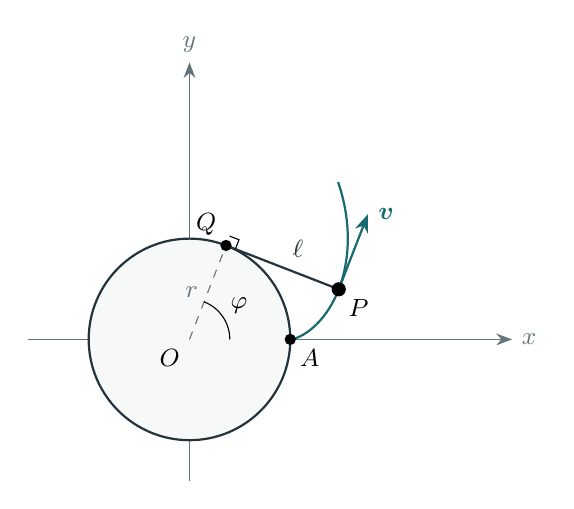
\begin{tikzpicture}[scale=1.28]
\draw[axis] (-1.6,0)--(3.2,0) node[right] {$x$};\draw[axis] (0,-1.4)--(0,2.75) node[above] {$y$};
\draw[object,fill=rulegray!18] (0,0) circle (1);
\draw[traj,domain=0:1.9,samples=90] plot({cos(\x r)+\x*sin(\x r)},{sin(\x r)-\x*cos(\x r)});
\coordinate (Q) at ({cos(1.2 r)},{sin(1.2 r)});
\coordinate (P) at ({cos(1.2 r)+1.2*sin(1.2 r)},{sin(1.2 r)-1.2*cos(1.2 r)});
\draw[object] (Q)--(P) node[midway,above right] {$\ell$};
\draw[guide] (0,0)--(Q) node[midway,left] {$r$};
\draw[motion] (P)--($(P)+(.29,.746)$) node[right] {$\vect v$};
\fill (Q) circle(1.6pt);\fill (P) circle(2pt);\fill (1,0) circle(1.6pt);
\node[above left] at (Q) {$Q$};\node[below right] at (P) {$P$};\node[below right] at (1,0) {$A$};\node[below left] at (0,0) {$O$};
\draw (.4,0) arc(0:68.755:.4);\node at (.49,.34) {$\varphi$};
\draw[thin] ($(Q)+(.093,-.036)$)--($(Q)+(.129,.057)$)--($(Q)+(.036,.093)$);
\end{tikzpicture}
\figcaption{图 1.9\quad $Q$ 为瞬时切点，$QP$ 为解开的直线段；图中选取逆时针展开支。}
\end{center}

\Needspace{5\baselineskip}\subsection*{解答}

设当前切点为 $Q$，小球为 $P$，外露绷直线段长度为 $\ell$。以圆心为原点，初始接触半径为 $x$ 轴正向；选取解线方向使切点沿圆周逆时针移动，转角记为 $\varphi$。另一侧解线得到镜像轨迹。
\begin{center}\begin{minipage}{\linewidth}\centering\begin{tikzpicture}

\draw[object] (0,0) circle(1);\node[below left] at (0,0) {$O$};
\coordinate (Q) at ({cos(1 r)},{sin(1 r)});\coordinate (P) at ({cos(1 r)+sin(1 r)},{sin(1 r)-cos(1 r)});
\draw[guide] (0,0)--(Q) node[midway,left] {$r$};\draw[object] (Q)--(P) node[midway,below] {$\ell$};
\draw[motion] (P)--($(P)+(.54,.84)$) node[right] {$\vect v$};
\draw[force] (P)--($(P)+(-.67,.43)$) node[midway,above] {$\vect a$};
\fill (Q) circle(1.8pt);\fill (P) circle(2pt);\node[above left] at (Q) {$Q$};\node[below right] at (P) {$P$};
\draw (.35,0) arc(0:57.296:.35);\node at (.57,.29) {$\varphi$};
\node[align=left] at (5.2,1.0) {$\vect v\perp QP$，张力不做功\\曲率半径为 $\ell$\\$a=v^2/\ell$，指向 $Q$};

\end{tikzpicture}
\figcaption{解图 1.9A\quad 张力改变速度方向；图中绳段长度 $\ell$ 决定法向加速度。}
\end{minipage}\end{center}
\subsubsection*{无滑动约束与速率不变}
解图 1.9A 中，圆柱上少缠绕的弧长等于新增外露线长，故
\[
\ell=r\varphi,\qquad\dd\ell=r\dd\varphi.
\]
令 $\vect e_r=(\cos\varphi,\sin\varphi)$、$\vect e_\varphi=(-\sin\varphi,\cos\varphi)$，则
\[
\vect{OQ}=r\vect e_r,\qquad
\vect{QP}=-\ell\vect e_\varphi,
\quad\vect{OP}=r\vect e_r-r\varphi\vect e_\varphi.
\]
利用 $\dd\vect e_r/\dd\varphi=\vect e_\varphi$、$\dd\vect e_\varphi/\dd\varphi=-\vect e_r$，对位置求导，
\[
\frac{\dd\vect{OP}}{\dd\varphi}
=r\vect e_\varphi-r\vect e_\varphi+r\varphi\vect e_r
=\ell\vect e_r.
\]
所以小球速度垂直于直线段 $QP$。张力沿 $PQ$，始终与速度垂直，不做功，因而小球速率恒为初速 $v$。$Q$ 是当前小球位置的曲率中心，随后沿圆柱移动。
\subsubsection*{线长、转角与时间}
由位置微分的长度，$\dd s=\ell\dd\varphi$。又 $\dd s=v\dd t$，因此
\[
v\dd t=\ell\dd\varphi=\frac{\ell}{r}\dd\ell.
\]
从 $\ell=0,t=0$ 积分，
\[
\frac{\ell^2}{2}=rvt,
\qquad\boxed{\ell(t)=\sqrt{2rvt}},\qquad
\boxed{\varphi(t)=\sqrt{\frac{2vt}{r}}}.
\]
\subsubsection*{加速度大小、方向与曲率}
速度矢量为 $\vect v=v\vect e_r$。对时间求导，
\[
\vect a=v\dot\varphi\vect e_\varphi
=\frac{v^2}{\ell}\vect e_\varphi.
\]
而 $\vect{PQ}=\ell\vect e_\varphi$，所以加速度由小球指向当前切点。其大小为
\[
\boxed{a(t)=\frac{v^2}{\sqrt{2rvt}}
=\frac{v^{3/2}}{\sqrt{2rt}}},\qquad t>0.
\]
轨迹切线方向转过 $\dd\varphi$ 时走过弧长 $\dd s=\ell\dd\varphi$，故曲率半径 $\rho_c=\dd s/\dd\varphi=\ell$，与 $a=v^2/\rho_c$ 一致。
\begin{center}\begin{minipage}{\linewidth}\centering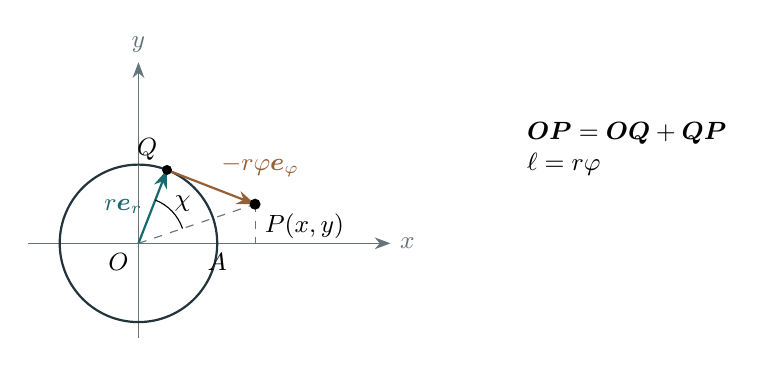
\begin{tikzpicture}

\draw[axis] (-1.4,0)--(3.2,0) node[right] {$x$};\draw[axis] (0,-1.2)--(0,2.3) node[above] {$y$};
\draw[object] (0,0) circle(1);
\coordinate (Q) at ({cos(1.2 r)},{sin(1.2 r)});\coordinate (P) at ({cos(1.2 r)+1.2*sin(1.2 r)},{sin(1.2 r)-1.2*cos(1.2 r)});
\draw[motion] (0,0)--(Q) node[midway,left] {$r\vect e_r$};
\draw[force] (Q)--(P) node[midway,above right] {$-r\varphi\vect e_\varphi$};
\draw[guide] (0,0)--(P);\draw[guide] (P)--({cos(1.2 r)+1.2*sin(1.2 r)},0);
\draw[thin] ({.59*cos(18.560)},{.59*sin(18.560)}) arc[start angle=18.560,end angle=68.755,radius=.59];
\node at (.56,.51) {$\chi$};
\fill (Q) circle(1.8pt);\fill (P) circle(2pt);\node[above left] at (Q) {$Q$};\node[below right] at (P) {$P(x,y)$};
\node[below left] at (0,0) {$O$};\node[below] at (1,0) {$A$};
\node[align=left] at (6.2,1.2) {$\vect{OP}=\vect{OQ}+\vect{QP}$\\$\ell=r\varphi$};

\end{tikzpicture}
\figcaption{解图 1.9B\quad 小球位置由半径矢量与展开绳段矢量相加得到；两矢量互相垂直。}
\end{minipage}\end{center}
\subsubsection*{展开位置得到参数轨迹}
将两基矢分量代入 $\vect{OP}$，
\[
\boxed{\begin{aligned}
x&=r(\cos\varphi+\varphi\sin\varphi),\\
y&=r(\sin\varphi-\varphi\cos\varphi),
\end{aligned}\qquad\varphi=\sqrt{\frac{2vt}{r}}}.
\]
解图 1.9B 中，切点到小球的连线沿圆柱切线，随切点移动形成圆的渐开线。斜边 $|\vect{OP}|=r\sqrt{1+\varphi^2}$ 给小球到圆心的距离，直角边 $QP=\ell$ 则是该点的曲率半径。

当 $t\to0^+$ 时 $\ell\to0$、$a\to\infty$；初始零外露线长使理想约束在起点产生奇点，所以加速度公式只在 $t>0$ 使用。位置与速度有有限的右极限：$P\to(r,0)$、$\vect v\to(v,0)$，符合题设的向外初速度。若可解开的总长为$\ell_{\max}$，这段运动在$\ell(t)=\ell_{\max}$时结束。
\subsubsection*{用直角三角形展开轨迹的另一方法}
解图1.9B中$OQ\perp QP$。设$\rho=OP$，
并以$\chi$表示$OQ$与$OP$的夹角，则直角三角形给出
\[
\rho=\sqrt{r^2+\ell^2}=r\sqrt{1+\varphi^2},\qquad
\cos\chi=\frac r\rho,\quad \sin\chi=\frac{\ell}{\rho}.
\]
当前$OP$相对于$x$轴的角度为$\varphi-\chi$，故
\[
\begin{aligned}
x&=\rho\cos(\varphi-\chi)
=r\cos\varphi+\ell\sin\varphi,\\
y&=\rho\sin(\varphi-\chi)
=r\sin\varphi-\ell\cos\varphi.
\end{aligned}
\]
将$\ell=r\varphi$代入两个投影式，所得$x$、$y$就是解图1.9B所示的渐开线坐标。
这里$\rho=OP$用于投影求坐标，$\ell=QP$由$\dd s/\dd\varphi$进入法向加速度。
速率恒定还意味着$\dd\vect v$只表示方向变化：
$|\dd\vect v|=v\,\dd\varphi$，因而
$a=v\dot\varphi=v\dot\ell/r$；
由$\dot\ell=\sqrt{rv/(2t)}$同样得到前面的法向加速度。


\Needspace{18\baselineskip}

\pdfbookmark[2]{第 10 题 旋转杆上小环的阿基米德螺线}{q10}

\section*{第 10 题\quad 旋转杆上小环的阿基米德螺线}

\tagline{M-01-10}

一根足够长的细杆在固定平面内绕端点 $O$ 以恒定角速度 $\omega>0$ 逆时针旋转。小环可看作质点，沿杆向外的相对速率恒为 $v>0$。设 $t=0$ 时小环位于 $O$，杆沿 $x$ 轴正方向。
\begin{enumerate}
\item 证明小环轨迹为阿基米德螺线；
\item 求任意时刻的速度、加速度向量及其大小；
\item 定性画出加速度在轨迹切向与法向的分量，并说明各自作用。
\end{enumerate}

\begin{center}
\begin{minipage}{\linewidth}\centering
\begin{tikzpicture}[scale=1.1]
\draw[axis] (-2.1,0)--(3.3,0) node[right] {$x$};\draw[axis] (0,-1.9)--(0,3.3) node[above] {$y$};
\draw[traj,domain=0:5.4,samples=120] plot({.45*\x*cos(\x r)},{.45*\x*sin(\x r)});
\coordinate (P) at ({.45*1.1*cos(1.1 r)},{.45*1.1*sin(1.1 r)});
\draw[object,line width=1.2pt] (0,0)--({2.9*cos(1.1 r)},{2.9*sin(1.1 r)});
\filldraw[fill=white,draw=ink,thick] (P) circle(2.4pt);\node[right] at (P) {$P$};
\draw[motion] (.48,.94)--(.94,1.85) node[right] {$v\vect e_r$};
\draw (.34,0) arc(0:63.025:.34);\node at (.65,.2) {$\varphi$};
\draw[motion] (.8,-.45) arc(-29:22:.92);\node[right] at (.98,-.3) {$\omega$};
\node[below left] at (0,0) {$O$};\node[color=muted] at (2.35,2.5) {转动杆};
\end{tikzpicture}
\figcaption{图 1.10\quad 小环沿杆向外运动，同时随杆转动；箭头 $v\vect e_r$ 表示相对速度。}
\end{minipage}
\end{center}

\Needspace{5\baselineskip}\subsection*{解答}

取逆时针角度为正。小环沿杆向外的相对速率为 $v$，故 $r=vt$；杆匀角速转动，故 $\varphi=\omega t$。题图 1.10 中每转过相同角度，小环的半径增加相同量。
\subsubsection*{轨迹与极坐标基矢}
消去时间，
\[
\boxed{r=\frac v\omega\varphi},\qquad \varphi\geq0,
\]
这是阿基米德螺线。直角坐标参数式为
\[
x=vt\cos\omega t,\qquad y=vt\sin\omega t.
\]
令 $\vect e_r=(\cos\varphi,\sin\varphi)$、$\vect e_\varphi=(-\sin\varphi,\cos\varphi)$。这些基矢随杆转动，满足
\[
\dot{\vect e}_r=\omega\vect e_\varphi,\qquad
\dot{\vect e}_\varphi=-\omega\vect e_r.
\]
\subsubsection*{速度与加速度矢量}
对位置 $\vect r=r\vect e_r$ 求导，
\[
\vect V=\dot r\vect e_r+r\omega\vect e_\varphi
=\boxed{v\vect e_r+v\omega t\vect e_\varphi}.
\]
前一项是沿杆相对速度，后一项是随杆转动的牵连速度。再求导，
\[
\vect a=v\omega\vect e_\varphi
+v\omega\vect e_\varphi-v\omega^2t\vect e_r
=\boxed{-v\omega^2t\vect e_r+2v\omega\vect e_\varphi}.
\]
径向速度 $v\vect e_r$ 的方向随杆转动，求导给出第一个 $v\omega\vect e_\varphi$。牵连速度的大小 $r\omega$ 随半径增加，求导给出第二个同向分量；其方向转动则给出 $-r\omega^2\vect e_r$。解图1.10A 左图画速度的两个箭头，右图画由这三项合成的加速度。
\begin{center}\begin{minipage}{\linewidth}\centering\begin{tikzpicture}

\begin{scope}
\draw[axis] (-.3,0)--(3,0) node[right] {$\vect e_r$};\draw[axis] (0,-.2)--(0,3) node[above] {$\vect e_\varphi$};
\draw[motion] (0,0)--(1.7,0) node[midway,below] {$v$};\draw[motion] (0,0)--(0,1.7) node[midway,left] {$r\omega$};
\draw[force] (0,0)--(1.7,1.7) node[above right] {$\vect V$};\draw[guide] (1.7,0)--(1.7,1.7)--(0,1.7);
\node[below left] at (0,0) {$P$};\node at (1.2,3.35) {绝对速度};
\end{scope}
\begin{scope}[xshift=6.5cm]
\draw[axis] (-2.1,0)--(2,0) node[right] {$\vect e_r$};\draw[axis] (0,-.2)--(0,3) node[above] {$\vect e_\varphi$};
\draw[motion] (0,0)--(-1.1,0) node[midway,below] {$-r\omega^2$};\draw[motion] (0,0)--(0,2.2) node[midway,right] {$2v\omega$};
\draw[force] (0,0)--(-1.1,2.2) node[above left] {$\vect a$};\draw[guide] (-1.1,0)--(-1.1,2.2)--(0,2.2);
\node[below left] at (0,0) {$P$};\node at (-.3,3.35) {极坐标加速度};
\end{scope}

\end{tikzpicture}
\figcaption{解图 1.10A\quad 在 $\omega t=1$ 时示意矢量分解。左图沿轨迹切线的总速度包含径向与横向分量。}
\end{minipage}\end{center}
两正交分量平方相加得
\[
\boxed{V=v\sqrt{1+\omega^2t^2}},\qquad
\boxed{a=v\omega\sqrt{4+\omega^2t^2}}.
\]
直角坐标中的矢量可写为
\[
\begin{aligned}
\vect V={}&v(\cos\omega t-\omega t\sin\omega t)\vect e_x
+v(\sin\omega t+\omega t\cos\omega t)\vect e_y,\\
\vect a={}&(-v\omega^2t\cos\omega t-2v\omega\sin\omega t)\vect e_x\\
&+(-v\omega^2t\sin\omega t+2v\omega\cos\omega t)\vect e_y.
\end{aligned}
\]
在直角坐标中，$v t$ 和三角函数分别求导。一次求导得到速度，再求导时两次出现 $v\omega$，它们与解图1.10A 中的两个横向贡献一一对应。
\subsubsection*{自然坐标中的切向与法向分量}
记 $s=\omega t$。轨迹切向单位矢量和朝曲率中心的法向单位矢量为
\[
\vect e_\tau=\frac{\vect e_r+s\vect e_\varphi}{\sqrt{1+s^2}},\qquad
\vect e_n=\frac{-s\vect e_r+\vect e_\varphi}{\sqrt{1+s^2}}.
\]
\begin{center}\begin{minipage}{\linewidth}\centering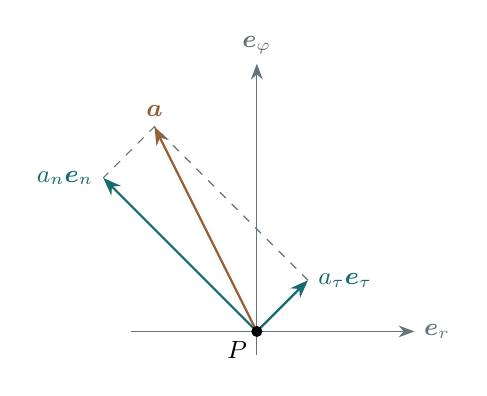
\begin{tikzpicture}

\coordinate (P) at (0,0);\coordinate (T) at (.65,.65);\coordinate (N) at (-1.95,1.95);
\draw[axis] (-1.6,0)--(2,0) node[right] {$\vect e_r$};\draw[axis] (0,-.3)--(0,3.4) node[above] {$\vect e_\varphi$};
\draw[motion] (P)--(T) node[right] {$a_\tau\vect e_\tau$};\draw[motion] (P)--(N) node[left] {$a_n\vect e_n$};
\draw[force] (P)--(-1.3,2.6) node[above] {$\vect a$};\draw[guide] (T)--(-1.3,2.6)--(N);
\fill (P) circle(2pt);\node[below left] at (P) {$P$};

\end{tikzpicture}
\figcaption{解图 1.10B\quad 在 $\omega t=1$ 时，把同一加速度改按轨迹切向、法向分解。切向改变速率，法向改变速度方向。}
\end{minipage}\end{center}
解图 1.10B 将同一加速度按轨迹切向、法向分解。投影到这两方向，或对速率求导，得到
\[
\boxed{a_\tau=\frac{\dd V}{\dd t}
=\frac{v\omega^2t}{\sqrt{1+\omega^2t^2}}},\qquad
\boxed{a_n=\frac{v\omega(2+\omega^2t^2)}{\sqrt{1+\omega^2t^2}}}.
\]
切向分量改变速率，法向分量使速度转向曲率中心。解图1.10B 的切线沿总速度，与杆有夹角。径向加速度沿杆向内，横向加速度沿转动方向；把两者投到切线上相加，所得 $a_\tau$ 在 $t>0$ 时为正，因而地面系速率增加。

在 $t=0$，$V=v$、$a_\tau=0$、$a_n=2v\omega$，加速度完全法向；此后速率增大，$a_\tau>0$。曲率半径为
\[
\rho_c=\frac{V^2}{a_n}
=\frac v\omega\frac{(1+\omega^2t^2)^{3/2}}{2+\omega^2t^2}.
\]
当 $\omega\to0$ 而 $t$ 固定时，速度趋于沿杆的 $v$，加速度趋于零，恢复直线匀速运动。
\subsubsection*{螺线的切线与曲率圆}
解图1.10A中的径向沿杆，而小环对地速度一般斜向杆的前侧。
解图1.10C把这两种方向放回轨迹，虚线圆在$P$处与螺线相切，
其圆心位于$P+\rho_c\vect e_n$。
切向单位矢量沿$\vect V$，法向单位矢量指向该圆心；
径向单位矢量则沿 $OP$，它与切向单位矢量的夹角满足 $\tan\angle(\vect e_r,\vect e_\tau)=s$。
\begin{center}\begin{minipage}{\linewidth}\centering
\begin{tikzpicture}
\coordinate (P) at (.5403,.8415);
\coordinate (K) at (-.3809,.6407);
\draw[axis] (-1.65,0)--(2.05,0) node[right] {$x$};
\draw[axis] (0,-.5)--(0,2.5) node[above] {$y$};
\draw[traj,domain=0:2,samples=100] plot({\x*cos(\x r)},{\x*sin(\x r)});
\draw[guide] (K) circle(.9428);
\draw[thin] (0,0)--(P);
\draw[force] (P)--(.8645,1.3464) node[right] {$\vect e_r$};
\draw[motion] (P)--(.391,1.526) node[above right] {$\vect e_\tau$};
\draw[motion] (P)--(-.144,.692) node[below left] {$\vect e_n$};
\fill (P) circle(1.8pt); \fill (K) circle(1.5pt);
\node[above right] at (P) {$P$}; \node[left] at (K) {$K$};
\node[below right] at (0,0) {$O$};
\node[align=left] at (5.4,1.25)
{$\omega t=1$，长度以$v/\omega$为单位\\
$PK=\rho_c=2\sqrt2/3$\\
虚线圆与轨迹在$P$处相切};
\end{tikzpicture}
\figcaption{解图1.10C\quad 螺线上的运动点与瞬时曲率圆；$K$是当前曲率中心。}
\end{minipage}\end{center}
例如$\omega t=1$时，
$\vect e_\tau=(\vect e_r+\vect e_\varphi)/\sqrt2$，
$\vect e_n=(-\vect e_r+\vect e_\varphi)/\sqrt2$。
将$\vect a=-v\omega\vect e_r+2v\omega\vect e_\varphi$分别点乘，
得到$a_\tau=v\omega/\sqrt2$、$a_n=3v\omega/\sqrt2$；
平方和仍为$5v^2\omega^2$，对应极坐标计算的同一个加速度大小。


\Needspace{18\baselineskip}

\pdfbookmark[2]{第 11 题 相对运动中的最短距离}{q11}

\section*{第 11 题\quad 相对运动中的最短距离}

\tagline{M-01-11}

质点甲、乙同时从 $A,B$ 出发，初始距离 $AB=\ell$。甲以速率 $v_1>0$ 沿 $AB$ 向右运动；乙以速率 $v_2>0$ 沿射线 $BC$ 运动。定义 $\alpha=\angle ABC$，即 $BA$ 与 $BC$ 的夹角，$0<\alpha<\pi$。两质点均作匀速直线运动，求出发以后（$t\geq0$）的最短距离。

\begin{center}\begin{minipage}{\linewidth}\centering\begin{tikzpicture}

\coordinate (A) at (0,0);\coordinate (B) at (5,0);\coordinate (C) at (2,2.25);
\draw[object] (A)--(B);\draw[guide] (B)--(C);
\fill (A) circle(2pt);\fill (B) circle(2pt);
\node[below] at (A) {$A$（甲）};\node[below right] at (B) {$B$（乙）};\node[above left] at (C) {$C$};
\draw[motion] (A)--(1.6,0) node[midway,above] {$v_1$};
\draw[motion] (B)--(3.4,1.2) node[midway,above right] {$v_2$};
\draw (4.2,0) arc(180:143.13:.8);\node at (4.05,.32) {$\alpha$};
\draw[thin,<->] (0,-.7)--(5,-.7) node[midway,below] {$\ell$};

\end{tikzpicture}
\figcaption{图 1.11\quad 角 $\alpha$ 从向左的射线 $BA$ 量起。图示为锐角情形。}
\end{minipage}\end{center}

\Needspace{5\baselineskip}\subsection*{解答}

取 $A$ 为初始原点，$AB$ 为 $x$ 轴正向，向上为 $y$ 正向。题图1.11 中 $\alpha$ 从向左的 $BA$ 量起。乙的速度与$x$正向夹角为$\pi-\alpha$，投影到$x,y$轴后得到
\[
\vect v_1=(v_1,0),\qquad
\vect v_2=(-v_2\cos\alpha,v_2\sin\alpha).
\]
\subsubsection*{转到随甲平移的参考系}
乙相对甲的速度为
\[
\vect w=\vect v_2-\vect v_1=(-p,q),\qquad
p=v_1+v_2\cos\alpha,\quad q=v_2\sin\alpha>0.
\]
在随甲平移的系中，甲固定于原点，乙的相对位置为
\[
\vect r(t)=(\ell-pt,qt),\qquad t\geq0.
\]
解图 1.11A 中乙沿相对速度确定的射线运动，求距离等价于求这条射线到原点的最近距离。
\begin{center}\begin{minipage}{\linewidth}\centering\begin{tikzpicture}

\coordinate (O) at (0,0);\coordinate (B) at (4,0);\coordinate (Q) at (.721,1.537);
\draw[axis] (-.4,0)--(4.7,0) node[right] {$x$};
\draw[traj] (B)--(-1.12,2.4);\draw[motion] (3.36,.3)--(2.08,.9) node[midway,above right] {$\vect w$};
\draw[object] (O)--(Q);\draw[guide] (O)--(B);
\pic[draw,angle radius=2.5mm] {right angle=O--Q--B};
\fill (O) circle(2pt);\fill (B) circle(2pt);\fill (Q) circle(2pt);
\node[below left] at (O) {甲};\node[below] at (B) {$B_0$};\node[above right] at (Q) {$Q$};
\node[left] at (.35,.8) {$r_{\min}$};
\node[align=left] at (7,1.7) {$\vect r(t)= (\ell-pt,qt)$\\垂足只有在未来的运动射线上\\才对应 $t\geq0$ 的最短距离。};

\end{tikzpicture}
\figcaption{解图 1.11A\quad 相对轨迹与最短距离。图中 $p>0$，垂足位于出发后的射线上。}
\end{minipage}\end{center}
\subsubsection*{在出发后的时段求距离最小值}
两质点距离平方为
\[
r^2(t)=(\ell-pt)^2+q^2t^2
=(p^2+q^2)t^2-2\ell pt+\ell^2.
\]
由于 $p^2+q^2>0$，配方得到
\[
r^2(t)=(p^2+q^2)\left(t-\frac{\ell p}{p^2+q^2}\right)^2
+\frac{\ell^2q^2}{p^2+q^2}.
\]
二次式顶点的横坐标为 $t_0=\ell p/(p^2+q^2)$，它对应直线上的垂足。实际运动从 $t=0$ 开始，须在半轴 $t\geq0$ 上选出使平方项最小的时间。

若 $p>0$，顶点在未来，距离先减小后增大，故
\[
t_* =\frac{\ell p}{p^2+q^2},\qquad
r_{\min}=\frac{\ell q}{\sqrt{p^2+q^2}}.
\]
若 $p\leq0$，则对 $t\geq0$ 有
\[
\frac{\dd r^2}{\dd t}=2(p^2+q^2)t-2\ell p\geq0,
\]
最近时刻就是出发时刻 $t_*=0$，最短距离为 $\ell$。因而完整结果为
\[
\boxed{t_* =\max\left(0,\frac{\ell(v_1+v_2\cos\alpha)}
{v_1^2+v_2^2+2v_1v_2\cos\alpha}\right)},
\]
\[
\boxed{r_{\min}=\begin{cases}
\dfrac{\ell v_2\sin\alpha}{\sqrt{v_1^2+v_2^2+2v_1v_2\cos\alpha}},
&v_1+v_2\cos\alpha>0,\\[5pt]
\ell,&v_1+v_2\cos\alpha\leq0.
\end{cases}}
\]
锐角时两物体的水平速度分量方向相反，故 $p>0$。钝角时乙的水平分量向右。当它达到或超过 $v_1$，就有 $p\leq0$，相对轨迹自 $B_0$ 起便朝远离原点的方向延伸。
\begin{center}\begin{minipage}{\linewidth}\centering\begin{tikzpicture}

\coordinate (O) at (0,0);\coordinate (B) at (3,0);\coordinate (Q) at (1.5,-1.5);
\draw[axis] (-.3,0)--(5.5,0) node[right] {$x$};
\draw[traj] (B)--(5,2);\draw[motion] (3.5,.5)--(4.3,1.3) node[midway,above left] {$\vect w$};
\draw[guide] (Q)--(B);\draw[object] (O)--(Q);\pic[draw,angle radius=3mm] {right angle=O--Q--B};
\fill (O) circle(2pt);\fill (B) circle(2pt);\fill (Q) circle(2pt);
\node[above left] at (O) {甲};\node[below right] at (B) {$B_0$};\node[below left] at (Q) {$Q$（过去）};
\draw[thin,<->] (0,.55)--(3,.55) node[midway,above] {$\ell=r_{\min}$};
\node[align=left] at (7.1,-1.2) {$p<0$，乙从开始就远离甲\\垂足对应 $t_0<0$\\未来射线的最近点为 $B_0$};

\end{tikzpicture}\figcaption{解图 1.11B\quad 垂足在过去的延长线上时，实际最短距离由初始端点给出。}
\end{minipage}\end{center}
解图 1.11B 的垂足落在相对射线的反向延长线上，对应负时间，实际最近点是出发位置 $B_0$。
\subsubsection*{用垂足和矢量公式解释}
当 $t_*>0$ 时，极值条件为
\[
\vect r(t_*)\cdot\vect w=0,
\]
即图中的相对位置垂直相对速度。整条直线到原点的距离还可写为
\[
\frac{|\vect r(0)\times\vect w|}{|\vect w|}
=\frac{\ell q}{\sqrt{p^2+q^2}}.
\]
这条叉乘式给的是点到\emph{直线}的垂距，只有垂足位于未来射线上时才是运动开始后的最短距离。题设 $q>0$，所以未来的最近距离仍大于零，两质点不会相遇。
\subsubsection*{从地面坐标到速度三角形}
在地面系中两位置分别为
\[
\vect r_1=(v_1t,0),\qquad
\vect r_2=(\ell-v_2t\cos\alpha,\ v_2t\sin\alpha).
\]
相减后得到随甲系中的 $\vect r(t)$，两地面速度也相减为相对速度 $\vect w$。从地面同时量得的两点间距离，正好等于这条相对位置矢量的长度。
若直接对距离$r(t)$求导，由题设$q>0$，距离始终为正，故
\[
\dot r=\frac{(p^2+q^2)t-\ell p}
{\sqrt{(\ell-pt)^2+q^2t^2}}.
\]
令分子为零得到同一 $t_0$。分母恒正，所以导数的符号由 $t-t_0$ 给出。在 $t_0\leq0$ 时，距离从出发起递增；在 $t_0>0$ 时，距离先减小，过 $t_0$ 后增大。
使用$r^2$配方只是省去了分母，保留了这套地面坐标求极值的全部条件。

若取$p>0$，把相对速度$\vect w=(-p,q)$与向左的初始连线方向之间的夹角记为$\alpha'$。
速度三角形给出
\[
w=\sqrt{v_1^2+v_2^2+2v_1v_2\cos\alpha},\qquad
\sin\alpha'=\frac{v_2\sin\alpha}{w}=\frac q w,\quad
\cos\alpha'=\frac p w>0.
\]
解图1.11A中，初始连线长为$\ell$，
垂线长为$\ell\sin\alpha'$，沿相对轨迹到垂足的距离为$\ell\cos\alpha'$。
因此$r_{\min}=\ell\sin\alpha'$，
$t_*=\ell\cos\alpha'/w=\ell p/w^2$。
这把三角函数法中的辅助角、速度三角形与实际垂足联系起来；
若 $p\leq0$，沿相对速度方向的有向投影为$\ell p/w\leq0$。图1.11B 中实际射线的最近点因而是 $B_0$，距离为 $\ell$。


\Needspace{18\baselineskip}

\pdfbookmark[2]{第 12 题 非均匀河流中的往返轨迹}{q12}

\section*{第 12 题\quad 非均匀河流中的往返轨迹}

\tagline{M-01-12}

宽为 $L$ 的河流沿 $x$ 轴正方向流动。以出发岸为 $y=0$、对岸为 $y=L$，流速大小与到较近河岸的距离成正比：两岸流速为零，河中心流速为 $v_0$。小船从原点出发，相对水以速率 $v_r$ 垂直水流驶向对岸；到 $y=L/4$ 时立即掉头，相对水以速率 $v_r/2$ 垂直水流返回出发岸。忽略掉头所需时间，求两段轨迹及返回点离出发点的距离。

\begin{center}\begin{minipage}{\linewidth}\centering\begin{tikzpicture}

\draw[object] (0,0)--(6,0);\draw[object] (0,3)--(6,3);
\draw[axis] (0,-.2)--(0,3.5) node[above] {$y$};\draw[axis] (0,0)--(6.5,0) node[right] {$x$};
\foreach \y/\a in {.3/.4,.75/1,1.5/2,2.25/1,2.7/.4}{\draw[motion] (3.4,\y)--({3.4+\a},\y);}
\node[right] at (5.4,1.5) {$v_0$};
\draw[guide] (0,.75)--(2.8,.75);\node[left] at (0,.75) {$L/4$};\node[left] at (0,3) {$L$};
\draw[motion] (.4,.12)--(.4,.65) node[left] {$v_r$};
\node[below left] at (0,0) {$O$};

\end{tikzpicture}
\figcaption{图 1.12\quad 流速沿河宽呈三角形分布；小船只在靠近出发岸的四分之一河宽内往返。}
\end{minipage}\end{center}

\Needspace{5\baselineskip}\subsection*{解答}

以沿岸方向为 $x$、横河方向为 $y$。由两岸流速为零、中心流速为 $v_0$，水流速度函数为
\[
u(y)=\begin{cases}
2v_0y/L,&0\leq y\leq L/2,\\
2v_0(L-y)/L,&L/2\leq y\leq L.
\end{cases}
\]
本题只到 $L/4$ 后返回，整个运动都使用第一段流速。船对地速度是水流速度与相对水速度的矢量和。
\subsubsection*{去程轨迹与掉头点}
去程相对水速度为 $v_r\vect e_y$，因此
\[
\dot x=\frac{2v_0}{L}y,\qquad\dot y=v_r.
\]
用 $y$ 作自变量，
\[
\frac{\dd x}{\dd y}=\frac{\dot x}{\dot y}
=\frac{2v_0y}{Lv_r},\qquad
x(y)=\int_0^y\frac{2v_0\eta}{Lv_r}\dd\eta.
\]
于是
\[
\boxed{x_{\text{去}}(y)=\frac{v_0y^2}{Lv_r}},
\quad0\leq y\leq\frac L4.
\]
掉头点 $P$ 的坐标为
\[
(x_P,y_P)=\left(\frac{v_0L}{16v_r},\frac L4\right),
\qquad t_P=\frac{L}{4v_r}.
\]
\subsubsection*{从掉头点写返程轨迹}
返程相对水速度是 $-v_r\vect e_y/2$。水流仍向下游，故
\[
\dot x=\frac{2v_0}{L}y,\qquad\dot y=-\frac{v_r}{2},
\qquad\frac{\dd x}{\dd y}=-\frac{4v_0y}{Lv_r}.
\]
以 $P$ 为返程初始点，积分为
\[
x(y)-x_P=\int_{L/4}^{y}-\frac{4v_0\eta}{Lv_r}\dd\eta
=-\frac{2v_0}{Lv_r}\left(y^2-\frac{L^2}{16}\right).
\]
所以
\[
\boxed{x_{\text{回}}(y)=\frac{3v_0L}{16v_r}
-\frac{2v_0y^2}{Lv_r}},\quad0\leq y\leq\frac L4.
\]
\begin{center}\begin{minipage}{\linewidth}\centering\begin{tikzpicture}

\draw[object] (-.3,0)--(4,0);\draw[axis] (0,-.2)--(0,2.65) node[above] {$y/L$};
\draw[axis] (-.2,0)--(4.3,0) node[right] {$16v_rx/(v_0L)$};
\draw[traj,domain=0:.25,samples=60] plot({16*\x*\x},{8*\x});
\draw[traj,domain=0:.25,samples=60] plot({3-32*\x*\x},{8*\x});
\draw[motion] (.16,.8)--(.36,1.2);\draw[motion] (1.72,1.6)--(2.28,1.2);
\fill (0,0) circle(2pt);\fill (1,2) circle(2pt);\fill (3,0) circle(2pt);
\node[below left] at (0,0) {$O$};\node[above] at (1,2) {$P$};\node[below] at (3,0) {$Q\,(3)$};
\draw[guide] (0,2)--(1,2);\node[left] at (0,2) {$1/4$};
\node[left] at (.36,1.35) {去程};\node[right] at (2.4,1.3) {返程};
\node[align=left] at (6.7,1.7) {返程横河速度减半，\\同一河宽内漂移更多。\\两段在 $P$ 连续相接。};

\end{tikzpicture}
\figcaption{解图 1.12A\quad 横坐标以 $v_0L/(16v_r)$ 为单位，图中箭头表示运动先后；返程继续向下游漂移。}
\end{minipage}\end{center}
解图1.12A 中两段曲线共用掉头点 $P$。沿返程箭头读图，$y$ 减小，$x$ 继续增大。积分上限从 $L/4$ 降到 $y$ 时，负的 $\dd x/\dd y$ 给出正的下游位移。到岸边后 $u(0)=0$，返回点为曲线与 $y=0$ 的交点。
\subsubsection*{返回点和两段漂移}
回到本岸时 $y=0$，故
\[
Q=\left(\frac{3v_0L}{16v_r},0\right),\qquad
\boxed{OQ=\frac{3v_0L}{16v_r}}.
\]
返程需时 $t_{\text{回}}=L/(2v_r)=2t_P$。两段都在 $0$ 与 $L/4$ 之间以恒定横河速率运动，时间平均流速均为端点流速的平均值 $v_0/4$。因此去程、返程漂移分别为
\[
\Delta x_{\text{去}}=\frac{v_0L}{16v_r},\qquad
\Delta x_{\text{回}}=\frac{v_0L}{8v_r},
\]
相加得到同一返回点距离。返程起点是 $P$，相对水速度反向且减半，水流速度保持向下游。
\subsubsection*{由掉头点确定积分常数和时间参数}
去程不定积分给$x=v_0y^2/(Lv_r)+C_1$。
出发时$(x,y)=(0,0)$，所以$C_1=0$；
返程则是$x=-2v_0y^2/(Lv_r)+C_2$，初始点已经移到解图1.12A中的$P$。
代入$P$的两坐标得
\[
C_2=x_P+\frac{2v_0}{Lv_r}y_P^2
=\frac{v_0L}{16v_r}+\frac{v_0L}{8v_r}
=\frac{3v_0L}{16v_r}.
\]
图1.12A 中，$C_2$ 是返程曲线在 $y=0$ 处的横坐标。两段共用点 $P$ 的条件确定了这个横坐标。

去程还有时间参数式
$y=v_rt$、$x=v_0v_rt^2/L$，$0\leq t\leq t_P$。
返程改用$s=t-t_P$，则
\[
y=\frac L4-\frac{v_r}{2}s,\qquad
x=x_P+\frac{v_0}{2}s-\frac{v_0v_r}{2L}s^2,
\qquad 0\leq s\leq\frac{L}{2v_r}.
\]
在$s=0$两段位置连续；横向速度从$v_r$变为$-v_r/2$，
顺水速度在掉头前后却同为$v_0/2$。
返回岸边时$y=0$、顺水速度也减为零，返回位置仍是$Q$。
返程的 $\dot y$ 为负，而 $\dot x$ 从 $v_0/2$ 均匀减到零。图1.12A 中两条箭头都指向下游，返程用时加倍，在同一流速区间内积累的下游位移也加倍。返程的横河加速度为零，顺水加速度为 $-v_0v_r/L$。这是把 $\dot y=-v_r/2$ 代入 $\dot u=(2v_0/L)\dot y$ 所得，表明越靠近岸边顺水速度越小。


\Needspace{18\baselineskip}

\pdfbookmark[2]{第 13 题 小船始终指向目标的河流轨迹}{q13}

\section*{第 13 题\quad 小船始终指向目标的河流轨迹}

\tagline{M-01-13}

笔直河流宽 $d$，水沿 $x$ 轴正方向以恒定速率 $v_0>0$ 流动。取对岸目标 $O$ 为极点，过 $O$ 顺水方向为极轴；出发岸位于 $y=d$。小船从 $A$ 出发，相对水的速率恒为 $v'>v_0$，且相对水的速度方向始终指向 $O$。已知 $OA=r_0$、$\angle AOP=\varphi_0$，其中 $OP$ 顺水，$0<\varphi_0<\pi$，$r_0\sin\varphi_0=d$。求轨迹；另求 $A$ 恰在 $O$ 正对岸时的结果。

\begin{center}\begin{minipage}{\linewidth}\centering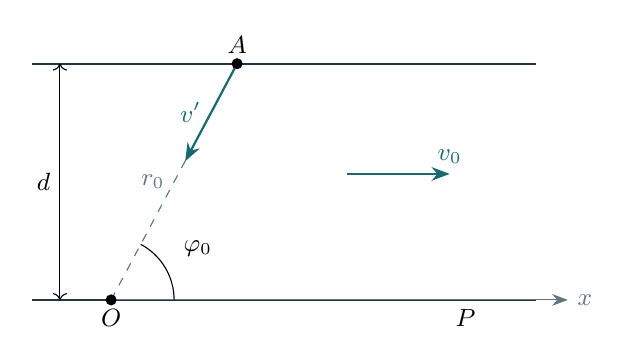
\begin{tikzpicture}

\draw[object] (-1,0)--(5.4,0);\draw[object] (-1,3)--(5.4,3);
\coordinate (O) at (0,0);\coordinate (A) at (1.6,3);
\draw[axis] (O)--(5.8,0) node[right] {$x$};\draw[guide] (O)--(A) node[midway,left] {$r_0$};
\draw[motion] (A)--(.94,1.76) node[midway,left] {$v'$};\draw[motion] (3,1.6)--(4.3,1.6) node[above] {$v_0$};
\draw (.8,0) arc(0:61.93:.8);\node at (1.1,.65) {$\varphi_0$};
\fill (O) circle(2pt);\fill (A) circle(2pt);\node[below] at (O) {$O$};\node[above] at (A) {$A$};\node[below] at (4.5,0) {$P$};
\draw[thin,<->] (-.65,0)--(-.65,3) node[midway,left] {$d$};

\end{tikzpicture}
\figcaption{图 1.13\quad 指向 $O$ 的是相对水速度；对地速度还要加上水流速度。}
\end{minipage}\end{center}

\Needspace{5\baselineskip}\subsection*{解答}

以固定目标 $O$ 为极点，顺水方向为极轴。船的位置为 $\vect r=r\vect e_r$，其中
\[
\vect e_r=(\cos\varphi,\sin\varphi),\qquad
\vect e_\varphi=(-\sin\varphi,\cos\varphi).
\]
相对水的速度始终指向目标，所以它等于 $-v'\vect e_r$。解图 1.13A 中水流的固定方向在这组随位置转动的基矢上有两个分量。
\begin{center}\begin{minipage}{\linewidth}\centering\begin{tikzpicture}

\coordinate (O) at (0,0);\coordinate (B) at (2.4,1.8);
\draw[axis] (0,0)--(4.6,0) node[right] {$x$};\draw[guide] (O)--(B) node[midway,above left] {$r$};
\draw[axis] (B)--(3.36,2.52) node[above right] {$\vect e_r$};\draw[axis] (B)--(1.68,2.76) node[above left] {$\vect e_\varphi$};
\draw[force] (B)--(1.12,.84) node[below left] {$-v'\vect e_r$};
\draw[motion] (B)--(3.5,1.8) node[right] {$v_0\vect e_x$};
\draw (.7,0) arc(0:36.87:.7);\node at (.95,.3) {$\varphi$};\fill (B) circle(2pt);
\node[align=left] at (7.2,2.1) {$\vect e_x=\cos\varphi\,\vect e_r-\sin\varphi\,\vect e_\varphi$\\径向：$\dot r=-v'+v_0\cos\varphi$\\横向：$r\dot\varphi=-v_0\sin\varphi$};

\end{tikzpicture}
\figcaption{解图 1.13A\quad 船向目标划行，水流在径向和横向都有投影。}
\end{minipage}\end{center}
\subsubsection*{合成速度并求轨迹微分方程}
水流速度为
\[
v_0\vect e_x=v_0\cos\varphi\vect e_r-v_0\sin\varphi\vect e_\varphi.
\]
因此船对地的径向、横向速度满足
\[
\boxed{\dot r=-v'+v_0\cos\varphi},\qquad
\boxed{r\dot\varphi=-v_0\sin\varphi}.
\]
因为 $v'>v_0$ 且 $0<\varphi<\pi$，$\dot r<0$、$\dot\varphi<0$：船逐渐接近目标，同时极角减小。用两方程相除消去时间，
\[
\frac{\dd r}{r}
=\frac{\dot r}{r\dot\varphi}\dd\varphi
=\left(\frac{v'}{v_0\sin\varphi}-\cot\varphi\right)\dd\varphi.
\]
\subsubsection*{用半角积分并代入初始条件}
记 $q=v'/v_0>1$，使用
\[
\int\frac{\dd\varphi}{\sin\varphi}=\ln\tan\frac\varphi2,
\qquad\int\cot\varphi\dd\varphi=\ln\sin\varphi.
\]
从 $(r_0,\varphi_0)$ 积分到 $(r,\varphi)$，得到
\[
\ln\frac r{r_0}
=q\ln\frac{\tan(\varphi/2)}{\tan(\varphi_0/2)}
-\ln\frac{\sin\varphi}{\sin\varphi_0}.
\]
两边取指数，轨迹为
\[
\boxed{\frac r{r_0}
=\left[\frac{\tan(\varphi/2)}{\tan(\varphi_0/2)}\right]^q
\frac{\sin\varphi_0}{\sin\varphi}},\qquad
0<\varphi\leq\varphi_0.
\]
轨迹的直角坐标由 $x=r\cos\varphi$、$y=r\sin\varphi$ 给出。初始时 $r=r_0$，且 $r_0\sin\varphi_0=d$，确在出发岸。
\subsubsection*{正对岸出发的轨迹与到达时刻}
目标恰在正对岸时，$r_0=d$、$\varphi_0=\pi/2$，所以
\[
\boxed{r(\varphi)=\frac d{\sin\varphi}
\left(\tan\frac\varphi2\right)^q}.
\]
\begin{center}\begin{minipage}{\linewidth}\centering\begin{tikzpicture}

\draw[object] (-.3,0)--(3.3,0);\draw[object] (-.3,3)--(3.3,3);
\draw[axis] (0,-.15)--(0,3.4) node[above] {$y$};\draw[axis] (0,0)--(3.6,0) node[right] {$x$};
\draw[traj,domain=0:1,samples=100] plot({1.5*(\x-\x*\x*\x)},{3*\x*\x});
\coordinate (P) at ({1/sqrt(3)},1);
\fill (0,0) circle(2pt);\fill (0,3) circle(2pt);\fill (P) circle(2pt);
\node[below left] at (0,0) {$O$};\node[above left] at (0,3) {$A$};\node[right] at (P) {$P$};
\draw[motion] (.432,1.92)--(.53,1.62);\draw[motion] (.4095,.27)--(.26,.1);
\draw[guide] (P)--({1/sqrt(3)},0);\draw[thin,<->] (-.5,0)--(-.5,3) node[midway,left] {$d$};
\draw[motion] (2.0,1.8)--(3.0,1.8) node[midway,above] {$v_0$};
\node[align=left] at (6.4,2.6) {$q=2$，$w=\tan(\varphi/2)$\\$x/d=(w-w^3)/2$\\$y/d=w^2$，$w:1\to0$};
\node[align=left] at (6.4,.8) {$P$ 为最远下游位置\\$x_P=d/(3\sqrt3)$，$y_P=d/3$};

\end{tikzpicture}\figcaption{解图 1.13B\quad 正对岸出发、相对水速率为水流速率两倍时的对地轨迹；箭头表示运动顺序。}
\end{minipage}\end{center}
解图 1.13B 绘出 $q=2$、正对岸出发的轨迹。船先向下游偏移，随后转向目标；图中的指向约束始终是相对水速度。

当 $\varphi\to0^+$，$\tan(\varphi/2)\sim\varphi/2$、$\sin\varphi\sim\varphi$，因此一般轨迹满足
\[
r\sim\frac{r_0\sin\varphi_0}{2^q[\tan(\varphi_0/2)]^q}
\varphi^{q-1}\longrightarrow0.
\]
因此船到目标的距离趋于零。再用解图1.13A的径向速度估计到达时间：
\[
v'-v_0\leq-\dot r\leq v'+v_0,
\qquad\frac{r_0}{v'+v_0}\leq t_*\leq\frac{r_0}{v'-v_0},
\]
因此在题设 $v'>v_0$ 下到达时间有限。终点坐标由$r\to0$与$\varphi\to0^+$的极限给出。沿解图1.13B的末段，船在下游一侧逐渐接近$O$，到达时位置为$(0,0)$。
\subsubsection*{半角积分和一般出发位置的到达时间}
半角积分可直接令$w=\tan(\varphi/2)$验证：
$\sin\varphi=2w/(1+w^2)$、
$\dd\varphi=2\dd w/(1+w^2)$，故
$\dd\varphi/\sin\varphi=\dd w/w$。
再与$\int\cot\varphi\,\dd\varphi=\ln\sin\varphi$合并，
并用初值作比，便得到上面的轨迹式。
在$0<\varphi\leq\varphi_0<\pi$内，$w$和$\sin\varphi$均为正，积分式使用正实数的对数。

还可按解图1.13A，记船的顺水坐标为$x=r\cos\varphi$。
对地速度的$x$分量为$\dot x=v_0-v'\cos\varphi$，
将它与径向速度组合得
\[
\frac{\dd}{\dd t}\left(r+\frac{v_0}{v'}x\right)
=-\frac{v'^2-v_0^2}{v'}.
\]
初始$x_0=r_0\cos\varphi_0$，到达$O$时$r=x=0$，因此
\[
\boxed{t_*=\frac{r_0(v'+v_0\cos\varphi_0)}{v'^2-v_0^2}}.
\]
它落在前面给出的上下时间界内。
正对岸时$\cos\varphi_0=0$、$r_0=d$，
简化为$t_*=dv'/(v'^2-v_0^2)$。
距离$r$始终缩短。对于正对岸出发的轨迹，顺水坐标$x$先增后减。解图1.13B的最远下游点$P$处$\dot x=0$，所以$\cos\varphi=1/q$。当$q=2$时，$\tan(\varphi/2)=1/\sqrt3$，代入图中的参数式得到$x_P=d/(3\sqrt3)$与$y_P=d/3$。


\Needspace{18\baselineskip}

\pdfbookmark[2]{第 14 题 纯滚动轮缘点速度}{q14}

\section*{第 14 题\quad 纯滚动轮缘点速度}

\tagline{M-01-14}

半径为 $r$ 的轮子在水平面上向右纯滚动。轮心速度为 $v_c$，轮的角速度大小为 $\omega$，转向为顺时针。设接触点为 $M$，轮缘点 $A$ 的位置角 $\theta$ 从 $CM$ 向逆时针量起，$0\leq\theta<2\pi$。求 $A$ 点对地的速度矢量、速率和方向。

\begin{center}\begin{minipage}{\linewidth}\centering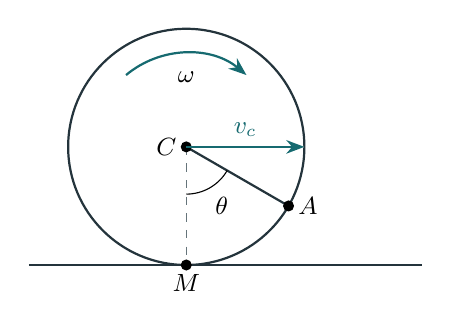
\begin{tikzpicture}

\coordinate (C) at (0,1.5);\coordinate (M) at (0,0);\coordinate (A) at (1.299,.75);
\draw[object] (-2,0)--(3,0);\draw[object] (C) circle(1.5);\draw[guide] (C)--(M);\draw[object] (C)--(A);
\fill (C) circle(2pt);\fill (A) circle(2pt);\fill (M) circle(2pt);
\node[left] at (C) {$C$};\node[below] at (M) {$M$};\node[right] at (A) {$A$};
\draw (0,.9) arc(-90:-30:.6);\node at (.45,.75) {$\theta$};
\draw[motion] (C)--(1.5,1.5) node[midway,above] {$v_c$};
\draw[motion] (-.765,2.412) arc(130:50:1.19);\node at (0,2.38) {$\omega$};

\end{tikzpicture}
\figcaption{图 1.14\quad 轮心平动与绕轮心顺时针转动同时存在。图中 $\theta=60^\circ$。}
\end{minipage}\end{center}

\Needspace{5\baselineskip}\subsection*{解答}

取水平向右为 $x$ 正向，竖直向上为 $y$ 正向，$\vect e_z$ 指向纸外。轮向右滚动，角速度矢量为 $\vect\omega=-\omega\vect e_z$。$\theta$ 从向下的半径 $CM$ 逆时针量起，所以
\[
\vect{CA}=r\sin\theta\vect e_x-r\cos\theta\vect e_y.
\]
\subsubsection*{由无滑动求平动与转动的关系}
接触材料点 $M$ 相对轮心的速度为 $-\omega r\vect e_x$。纯滚动要求它对地瞬时速度为零，因此
\[
\vect v_M=(v_c-\omega r)\vect e_x=0,
\qquad v_c=\omega r.
\]
\subsubsection*{速度叠加得到矢量与速率}
对任意轮缘点，刚体速度关系为
\[
\vect v_A=\vect v_C+\vect\omega\times\vect{CA}.
\]
把转动速度展开，
\[
\vect\omega\times\vect{CA}
=-\omega r\cos\theta\vect e_x-\omega r\sin\theta\vect e_y.
\]
利用纯滚动关系，得到
\[
\boxed{\vect v_A=v_c(1-\cos\theta)\vect e_x-v_c\sin\theta\vect e_y}.
\]
\begin{center}\begin{minipage}{\linewidth}\centering\begin{tikzpicture}

\coordinate (C) at (0,1.5);\coordinate (M) at (0,0);\coordinate (A) at (1.299,.75);
\draw[object] (-1.8,0)--(3,0);\draw[object] (C) circle(1.5);\draw[guide] (C)--(A);\draw[object] (M)--(A);
\draw[motion] (A)--(2.599,.75) node[above right] {$\vect v_C$};
\draw[force] (A)--(.649,-.376) node[below] {$\vect v_{A/C}$};
\draw[guide] (2.599,.75)--(1.949,-.376)--(.649,-.376);
\draw[motion] (A)--(1.949,-.376) node[below right] {$\vect v_A$};
\node[below left] at (M) {$M$};\node[above left] at (C) {$C$};\node[above] at (A) {$A$};
\node[align=left] at (6.1,1.8) {$\vect v_A\perp\vect{MA}$\\接地点可作速度的瞬时转动中心。\\顶部速率为 $2v_c$，底部为零。};

\end{tikzpicture}
\figcaption{解图 1.14A\quad 两等长速度矢量合成；合速度垂直于 $MA$。}
\end{minipage}\end{center}
解图 1.14A 将轮心平动速度与绕心转动速度相加。两矢量都长 $v_c$，合速度长度依位置而变：
\[
v_A^2=v_c^2[(1-\cos\theta)^2+\sin^2\theta]
=2v_c^2(1-\cos\theta).
\]
因此
\[
\boxed{v_A=2v_c\left|\sin\frac\theta2\right|}.
\]
在题图所用的 $0\leq\theta<2\pi$ 内，半角正弦非负。若把同一位置角写成负值，绝对值仍给出正确的弦长和速率。
\subsubsection*{瞬时转动中心给出方向}
由 $M$ 到 $A$ 的位置矢量为
\[
\vect{MA}=r\sin\theta\vect e_x+r(1-\cos\theta)\vect e_y.
\]
与 $\vect v_A$ 点乘得零，所以非接触点的速度垂直于 $MA$。其方向对应绕 $M$ 的瞬时顺时针转动，也可写为
\[
\vect v_A=\vect\omega\times\vect{MA},\qquad
MA=2r\left|\sin\frac\theta2\right|.
\]
因此瞬时中心法同样给出 $v_A=\omega MA$。更具体地，在 $0<\theta<2\pi$ 时，
\[
\frac{\vect v_A}{v_A}
=\sin\frac\theta2\vect e_x-\cos\frac\theta2\vect e_y.
\]
接地点 $\theta=0$ 速度为零，没有速度方向；最高点 $\theta=\pi$ 水平向右，速率 $2v_c$；右侧点 $\theta=\pi/2$ 向右下方，速率 $\sqrt2v_c$；左侧点 $\theta=3\pi/2$ 向右上方，速率同样为 $\sqrt2v_c$。

图1.14B 从同一个轮缘材料点出发，画出它随着轮子前进所描出的曲线。设轮心匀速前进，该点在$t=0$恰接地，令$\psi=\omega t$，则其摆线轨迹为
\[x_A=r(\psi-\sin\psi),\qquad y_A=r(1-\cos\psi).\]
求导得$\dot x_A=v_c(1-\cos\psi)$、$\dot y_A=v_c\sin\psi$，这里材料点随轮子顺时针转动，故 $\theta\equiv-\psi\pmod{2\pi}$，两个速度分量与前式一致。在$t=0$的接地瞬间，该材料点速度为零，加速度为$r\omega^2\boldsymbol e_y$。摆线起点的向上箭头画的正是这一加速度。
\begin{center}\begin{minipage}{0.94\linewidth}\centering
\begin{tikzpicture}[x=1cm,y=1cm]
\draw[->,color=muted] (-.25,0)--(4.9,0) node[right] {$x$};
\draw[->,color=muted] (0,-.1)--(0,1.9) node[above] {$y$};
\draw[thick,color=accent,domain=0:360,samples=100,variable=\t]
plot ({.65*(\t*pi/180-sin(\t))},{.65*(1-cos(\t))});
\fill (0,0) circle(1.5pt);\fill (4.084,0) circle(1.5pt);
\draw[->,thick,color=warm] (0,.08)--(0,.85) node[left] {$\boldsymbol a$};
\node[below] at (0,0) {$t=0$};\node[below] at (4.084,0) {$t=2\pi/\omega$};
\node at (2.1,1.65) {同一轮缘点的轨迹};
\end{tikzpicture}
\figcaption{解图1.14B\quad 两次接地之间的一拱摆线；尖点速度为零而加速度非零。}
\end{minipage}\end{center}
解图1.14A 比较同一时刻轮缘各点的速度，接地点 $M$ 随轮子前进，由不同材料点依次占据。解图1.14B 跟踪同一材料点的摆线，沿这条曲线对该点的速度随时间求导，便得到它的加速度。

\Needspace{18\baselineskip}

\pdfbookmark[2]{第 15 题 内滚圆盘接触点加速度}{q15}

\section*{第 15 题\quad 内滚圆盘接触点加速度}

\tagline{M-01-15}

半径 $R$ 的圆环固定，半径 $r<R$ 的圆盘沿圆环内侧无滑动滚动。圆盘中心 $C$ 绕环心 $O$ 以恒定角速度大小 $\Omega$ 运动。求圆盘上在当前时刻与圆环接触的材料点 $A$ 相对圆环的加速度大小和方向。

\begin{center}\begin{minipage}{\linewidth}\centering\begin{tikzpicture}

\coordinate (O) at (0,0);\coordinate (C) at (2,0);\coordinate (A) at (3,0);
\draw[object] (O) circle(3);\draw[guide] (O) circle(2);\draw[object] (C) circle(1);
\draw[object] (O)--(A);\node[below] at (1,0) {$R-r$};\node[below] at (2.5,0) {$r$};
\fill (O) circle(2pt);\fill (C) circle(2pt);\fill (A) circle(2pt);
\node[below left] at (O) {$O$};\node[above] at (C) {$C$};\node[right] at (A) {$A$};
\draw[motion] (1.1,0) arc(0:85:1.1) node[left] {$\Omega$};
\draw[motion] (2.24,.66) arc(70:-40:.7);\node at (2.6,-.8) {$\omega$};
\node[align=left] at (5.9,2) {圆环固定\\圆盘内滚\\当前接触材料点速度为零};

\end{tikzpicture}
\figcaption{图 1.15\quad 盘心逆时针绕 $O$ 运动时，圆盘绕自身中心顺时针转动。}
\end{minipage}\end{center}

\Needspace{5\baselineskip}\subsection*{解答}

设盘心轨道半径为 $\rho=R-r$。取 $\vect e_r$ 从环心 $O$ 指向盘心 $C$，$\vect e_\varphi$ 沿盘心逆时针运动方向；先取公转角速度为 $+\Omega\vect e_z$。相反转向给出相同的加速度大小与径向方向。
\subsubsection*{无滑动确定自转的方向与大小}
盘心速度为 $\vect v_C=\rho\Omega\vect e_\varphi$。当前接触材料点 $A$ 位于盘心外侧，故 $\vect{CA}=r\vect e_r$。若圆盘自身的角速度为 $\omega_s\vect e_z$，其对地速度满足
\[
\vect v_A=\rho\Omega\vect e_\varphi
+\omega_s\vect e_z\times r\vect e_r
=(\rho\Omega+r\omega_s)\vect e_\varphi.
\]
固定圆环的接触处速度为零，无滑动要求 $\vect v_A=0$，于是
\[
\boxed{\omega_s=-\frac{\rho}{r}\Omega}.
\]
负号说明圆盘对地自转与盘心公转反向，自转角速度大小为 $\omega=\rho\Omega/r$。式中的 $\omega_s$ 描述圆盘上的固定方向在地面系中的转动，代入刚体公式时直接使用这一角速度。
\subsubsection*{跟踪当前接触的同一个材料点}
盘心作匀速圆周运动，其加速度为
\[
\vect a_C=-\rho\Omega^2\vect e_r.
\]
$\Omega$ 恒定时 $\omega_s$ 也恒定，所以圆盘材料点的刚体加速度关系为
\[
\vect a_A=\vect a_C
+\vect\omega_s\times(\vect\omega_s\times\vect{CA}).
\]
自转贡献指向盘心，大小为 $r\omega_s^2$，与盘心的向心加速度同向。解图 1.15A 将两箭头平移画出，便于比较：
\begin{center}\begin{minipage}{\linewidth}\centering\begin{tikzpicture}

\coordinate (O) at (0,0);\coordinate (C) at (2.4,0);\coordinate (A) at (3.6,0);
\draw[object] (C) circle(1.2);\draw[guide] (O)--(A);\fill (O) circle(2pt);\fill (C) circle(2pt);\fill (A) circle(2pt);
\node[below] at (O) {$O$};\node[below] at (C) {$C$};\node[right] at (A) {$A$};
\draw[guide] (A)--(3.6,1.85);
\draw[force] (3.6,1.85)--(2.4,1.85) node[midway,above] {$\vect a_C$};
\draw[motion] (2.4,1.85)--(0,1.85) node[midway,above] {$\vect a_{A/C}$};
\draw[axis] (3.8,1.55)--(4.8,1.55) node[right] {$\vect e_r$};
\node[align=left] at (7,0) {两分量均朝向 $O$\\$\vect a_A=\vect a_C+\vect a_{A/C}$\\当前接触材料点沿 $AO$ 加速};

\end{tikzpicture}
\figcaption{解图 1.15A\quad 两支向内的加速度首尾相接。图取$\rho=2r$，绕心贡献是盘心贡献的两倍。}
\end{minipage}\end{center}
\[
\vect a_A=-\left[\rho\Omega^2+r\left(\frac\rho r\Omega\right)^2\right]\vect e_r
=-\frac{\rho(r+\rho)}r\Omega^2\vect e_r.
\]
由 $r+\rho=R$，最终
\[
\boxed{a_A=\frac{R(R-r)}r\Omega^2},\qquad
\boxed{\text{方向由接触点 }A\text{ 指向环心 }O}.
\]
式中 $R(R-r)/r$ 是长度，乘 $\Omega^2$ 得加速度量纲。
\subsubsection*{材料点和几何接触位置各自怎样运动}
无滑动使当前接触的材料点 $A$ 瞬时静止。圆盘继续滚动时，下一处接触由轮缘上的另一材料点承担。给当前的 $A$ 画一个标记，随后它沿图1.15A 的加速度方向起动并离开圆环。

圆环上几何接触位置为 $\vect{OA}_{\mathrm{geom}}=R\vect e_r$。当盘心方向改变时，该位置沿圆环以速率 $R\Omega$ 移动。被标记的材料点则在接触瞬间速度为零，它的加速度由盘心和绕心转动的两项给出。被标记的 $A$ 到了下一时刻已离开圆环，圆环上的接触位置由另一点占据。只看被跟踪点的速度，接触瞬间为零，随后向环内增大，正如抛体过最高点前后，竖直速度经过零而重力加速度始终向下。

当 $r=R/2$ 时，$\omega=\Omega$，两项加速度各为 $R\Omega^2/2$，相加得 $a_A=R\Omega^2$；当 $r\to R^-$ 时盘心轨道半径趋零，所求加速度也趋零。

\end{document}
